\documentclass{beamer}

\mode<presentation> {
\usetheme{CambridgeUS}
\usecolortheme{seagull}
\usefonttheme{default}
}

\usepackage{graphicx}
\usepackage{booktabs}
\usepackage{ragged2e}
\usepackage{lipsum}
\usepackage[export]{adjustbox}

%----------------------------------------------------------------------------------------
%	My Customized Settings
%----------------------------------------------------------------------------------------

\definecolor{UniBlue}{RGB}{83,121,170}
\definecolor{DarkGray}{RGB}{90,90,90}
\definecolor{LightGray}{RGB}{150,150,150}
\definecolor{TextGreen}{RGB}{115,155,15}
\definecolor{Ocean}{RGB}{23,142,189}

\setbeamercolor{normal}{fg=DarkGray}
\setbeamercolor{title}{fg=UniBlue}
\setbeamercolor{frametitle}{fg=UniBlue}
\setbeamercolor{structure}{fg=UniBlue}
\setbeamercolor{normal text}{fg=DarkGray,bg=white}
\setbeamercolor{section number projected}{bg=UniBlue,fg=white}

\setbeamertemplate{itemize item}{\scriptsize\raise1.25pt\hbox{\donotcoloroutermaths$\blacktriangleright$}}
\setbeamertemplate{itemize subitem}{\tiny\raise1.5pt\hbox{\donotcoloroutermaths$\bullet$}}
\setbeamertemplate{itemize subsubitem}{\tiny\raise1.5pt\hbox{\donotcoloroutermaths$\blacksqaure$}}
\setbeamercolor{itemize item}{fg=darkred}
\setbeamercolor{itemize subitem}{fg=TextGreen}
\setbeamercolor{itemize subbody}{fg=LightGray}

\setbeamertemplate{enumerate subitem}{\insertenumlabel.\insertsubenumlabel}
\setbeamertemplate{enumerate subsubitem}{\insertenumlabel.\insertsubenumlabel.\insertsubsubenumlabel}
\setbeamertemplate{enumerate mini template}{\insertenumlabel}

\setbeamertemplate{navigation symbols}{}

\newcommand\VeryLargeFont{\fontsize{30}{15}\selectfont}
\newcommand\LargeFont{\fontsize{15}{15}\selectfont}
\newcommand\TinyFont{\fontsize{6}{6}\selectfont}

\setbeamertemplate{frametitle} {
  \nointerlineskip
  \begin{beamercolorbox}[sep=0.15cm,ht=1.3em,wd=\paperwidth]{frametitle}
    \vbox{}\vskip-2ex
    \strut\insertframetitle\strut
    \vskip-0.8ex
  \end{beamercolorbox}
}

\defbeamertemplate*{title page}{customized}[1][] {
  \centering
  \bigskip
  \bigskip
  \bigskip
  \usebeamercolor[fg]{title}\insertsubtitle\par
  \usebeamerfont{title}\inserttitle\par
  \usebeamerfont{subtitle}
  \bigskip
  \usebeamercolor[fg]{normal}
  \usebeamerfont{author}\insertauthor\par
  \usebeamerfont{institute}\insertinstitute\par
  \usebeamerfont{date}\insertdate\par
  \bigskip
  \bigskip
  \bigskip
  \bigskip
  \bigskip
  \usebeamercolor[fg]{titlegraphic}\inserttitlegraphic
}

%----------------------------------------------------------------------------------------
%	TITLE PAGE
%----------------------------------------------------------------------------------------
\title[Introduction]{Introduction to Python}
\author{Parham Alvani}
\institute[AUT] {
  Amirkabir University of Technology \\
  \medskip
  {\small\tt parham.alvani@gmail.com}
}
\date{May 14, 2015}
\titlegraphic{\hspace*{5cm}
\includegraphics[width=2cm]{figs/aut_logo.jpeg}}

\begin{document}

\begin{frame}
\titlepage
\end{frame}

%----------------------------------------------------------------------------------------
%	PRESENTATION SLIDES
%----------------------------------------------------------------------------------------

%------------------------------------------------
\section{}
\subsection{}

%------------------------------------------------
\begin{frame}
\begin{columns}
\column{28em}
\vspace{2cm}
\begin{block}{\centering\textcolor{darkred}{what is python...}}
\justifying
Python is a high-level, interpreted, interactive and object-oriented scripting language. Python is designed to be highly readable..\\
\end{block}
\end{columns}
\vspace{.75cm}
\hspace*{8.5cm}
\includegraphics[width=3cm]{figs/python.jpeg}
\end{frame}

%------------------------------------------------
\begin{frame}
\frametitle{Variable Types}
\begin{columns}[c]
	\column{30em}
	\begin{itemize}
		\justifying
		\item Numbers
		\item String
		\item List
		\item Tuple
		\item Dictionary
	\end{itemize}
\end{columns}
\end{frame}

%------------------------------------------------
\begin{frame}
\begin{columns}
\column{28em}
\vspace{2cm}
\begin{block}{\centering\textcolor{darkred}{..., but there are problems with relying on data too much.}}
\justifying
Not everything that can be counted counts, and not everything that counts can be counted.\\
\vspace{.2cm}
\hspace*{8.5cm}\footnotesize{- Albert Einstein}
\end{block}
\end{columns}
\vspace{.75cm}
\hspace*{8.5cm}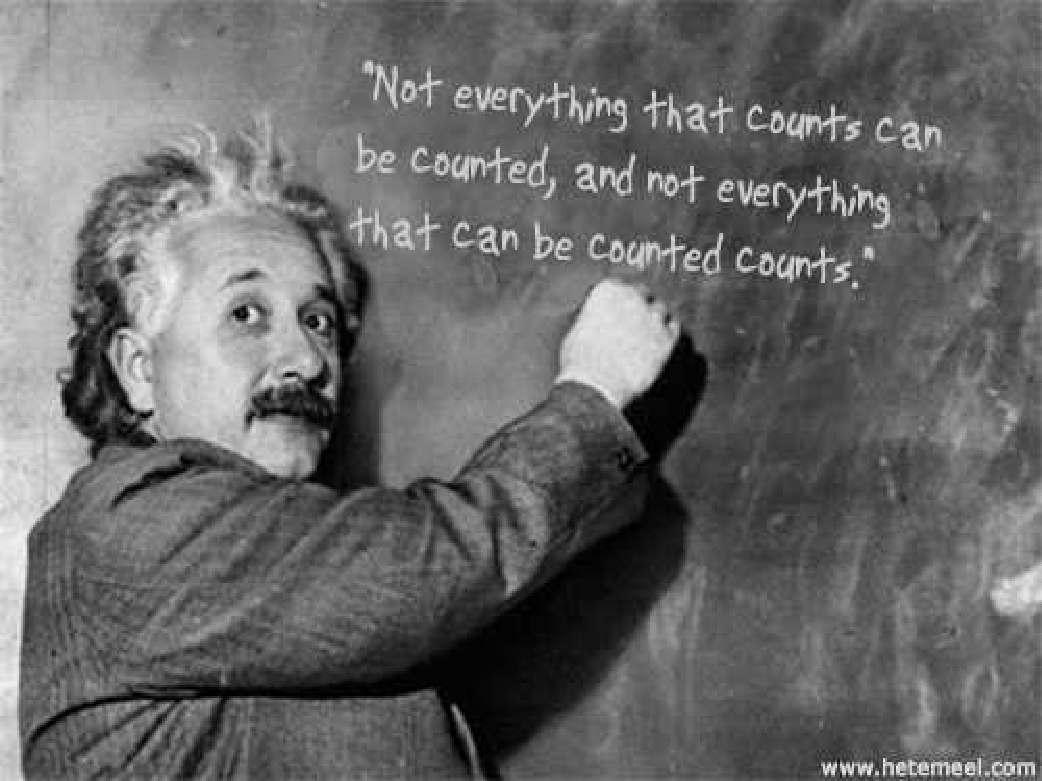
\includegraphics[width=3cm]{figs/einstein.pdf}
\end{frame}

%------------------------------------------------
\begin{frame}
\begin{columns}
\column{25em}
\vspace{2cm}
\begin{block}{\centering\textcolor{darkred}{Data is a treasure ..., except when it is not.}}
\justifying
Getting information off the Internet is like taking a drink from a fire hose.\\
\vspace{.2cm}
\hspace*{7.2cm}\footnotesize{- Mitchell Kapor}
\end{block}
\end{columns}
\vspace{.75cm}
\hspace*{9cm}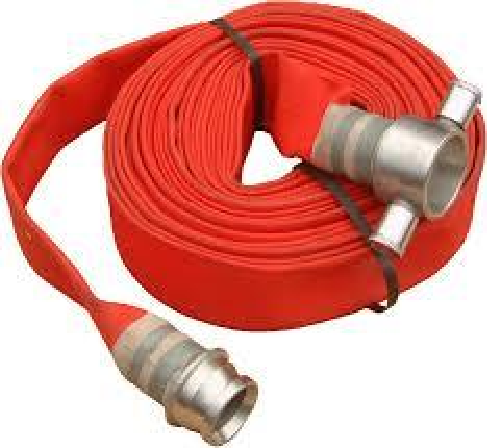
\includegraphics[width=2.5cm]{figs/firehose.pdf}
\end{frame}

%------------------------------------------------
\begin{frame}
\begin{columns}
\column{28em}
\vspace{2cm}
\begin{block}{\centering\textcolor{darkred}{However, any data is better than none.}}
\justifying
An approximate answer to the right problem is worth a good deal more than an exact answer to an approximate problem.\\
\vspace{.2cm}
\hspace*{8.7cm}\footnotesize{- John Tukey}
\end{block}
\end{columns}
\vspace{.75cm}
\hspace*{8cm}
\includegraphics[width=4cm]{figs/deal.pdf}
\end{frame}

%------------------------------------------------
\begin{frame}
\frametitle{Big Data, the Noam Chomsky Way}
\hspace*{9cm}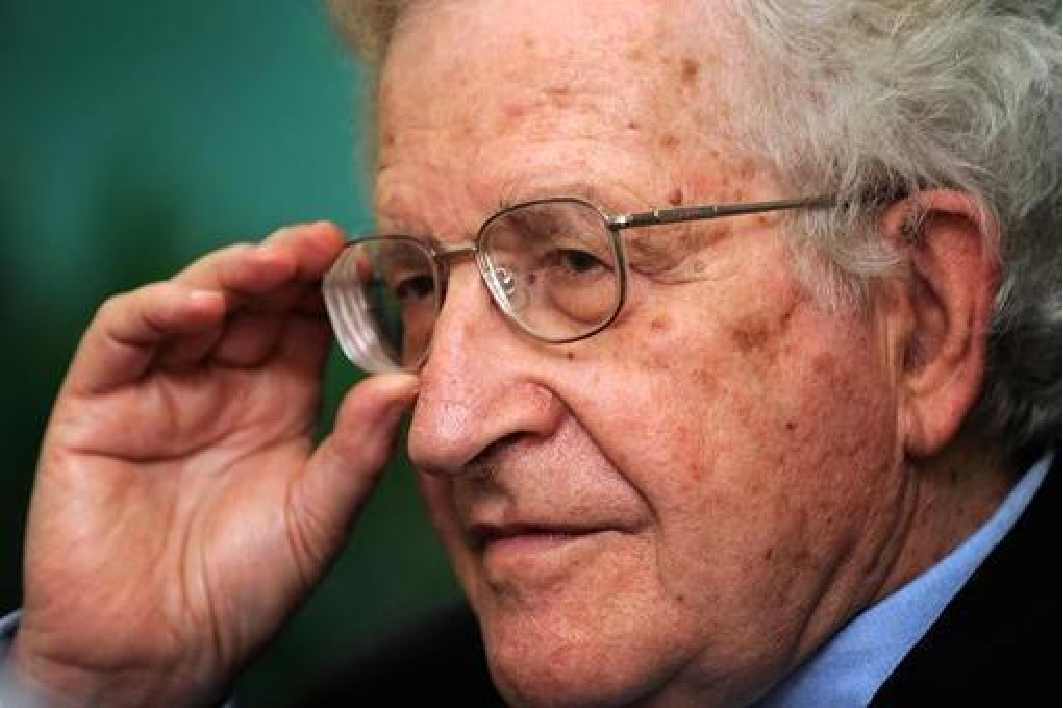
\includegraphics[width=2.5cm]{figs/chamsky.pdf}
\begin{columns}[c] 
\column{26em}
\begin{block}{}
\justifying
{\scriptsize Big data is a step forward. But, our problems are not lack of access to data, but understanding them. [Big data] is very useful if I want to find out something without going to the library, but I have to understand it, and that's the problem.}
\end{block}
\pause
\centering
\textcolor{Ocean}{Hmmm, not very much Chomsky-ish ..., but wait!}
\pause
\begin{block}{}
\centering
\justifying
{\scriptsize We can be confident that any system of power - whether it's the state, Google, or whatever - is going to use the best available technology to control, to dominate, and to maximize their power. And they'll want to do it in secret.}
\end{block}
\centering
\textcolor{darkred}{Now that's sounding more like Chomsky.}
\end{columns}
\end{frame}

%------------------------------------------------
\begin{frame}
\frametitle{They Want to Do It In Secret ...}
\begin{columns}
\column{17em}
\vspace{2cm}
\begin{block}{}
\centering
The truth cannot stay hidden forever!
\end{block}
\end{columns}
\vspace{.75cm}
\hspace*{9cm}\includegraphics[width=2cm]{figs/snowden.pdf}
\end{frame}

%------------------------------------------------
\begin{frame}
\vspace{1cm}
\Huge{\centerline{\usebeamercolor[fg]{title}A Brief History of}}
\Huge{\centerline{\usebeamercolor[fg]{title}Data Management!}}
\end{frame}

%------------------------------------------------
\begin{frame}
\frametitle{4000 B.C}
\begin{columns}[c] 
\column{30em}
\begin{itemize}
  \justifying
  \item Manual recording
  \item From tablets to papyrus, to parchment, and then to paper
\end{itemize}
\end{columns}
\vspace{0.5cm}
\hspace*{3.5cm}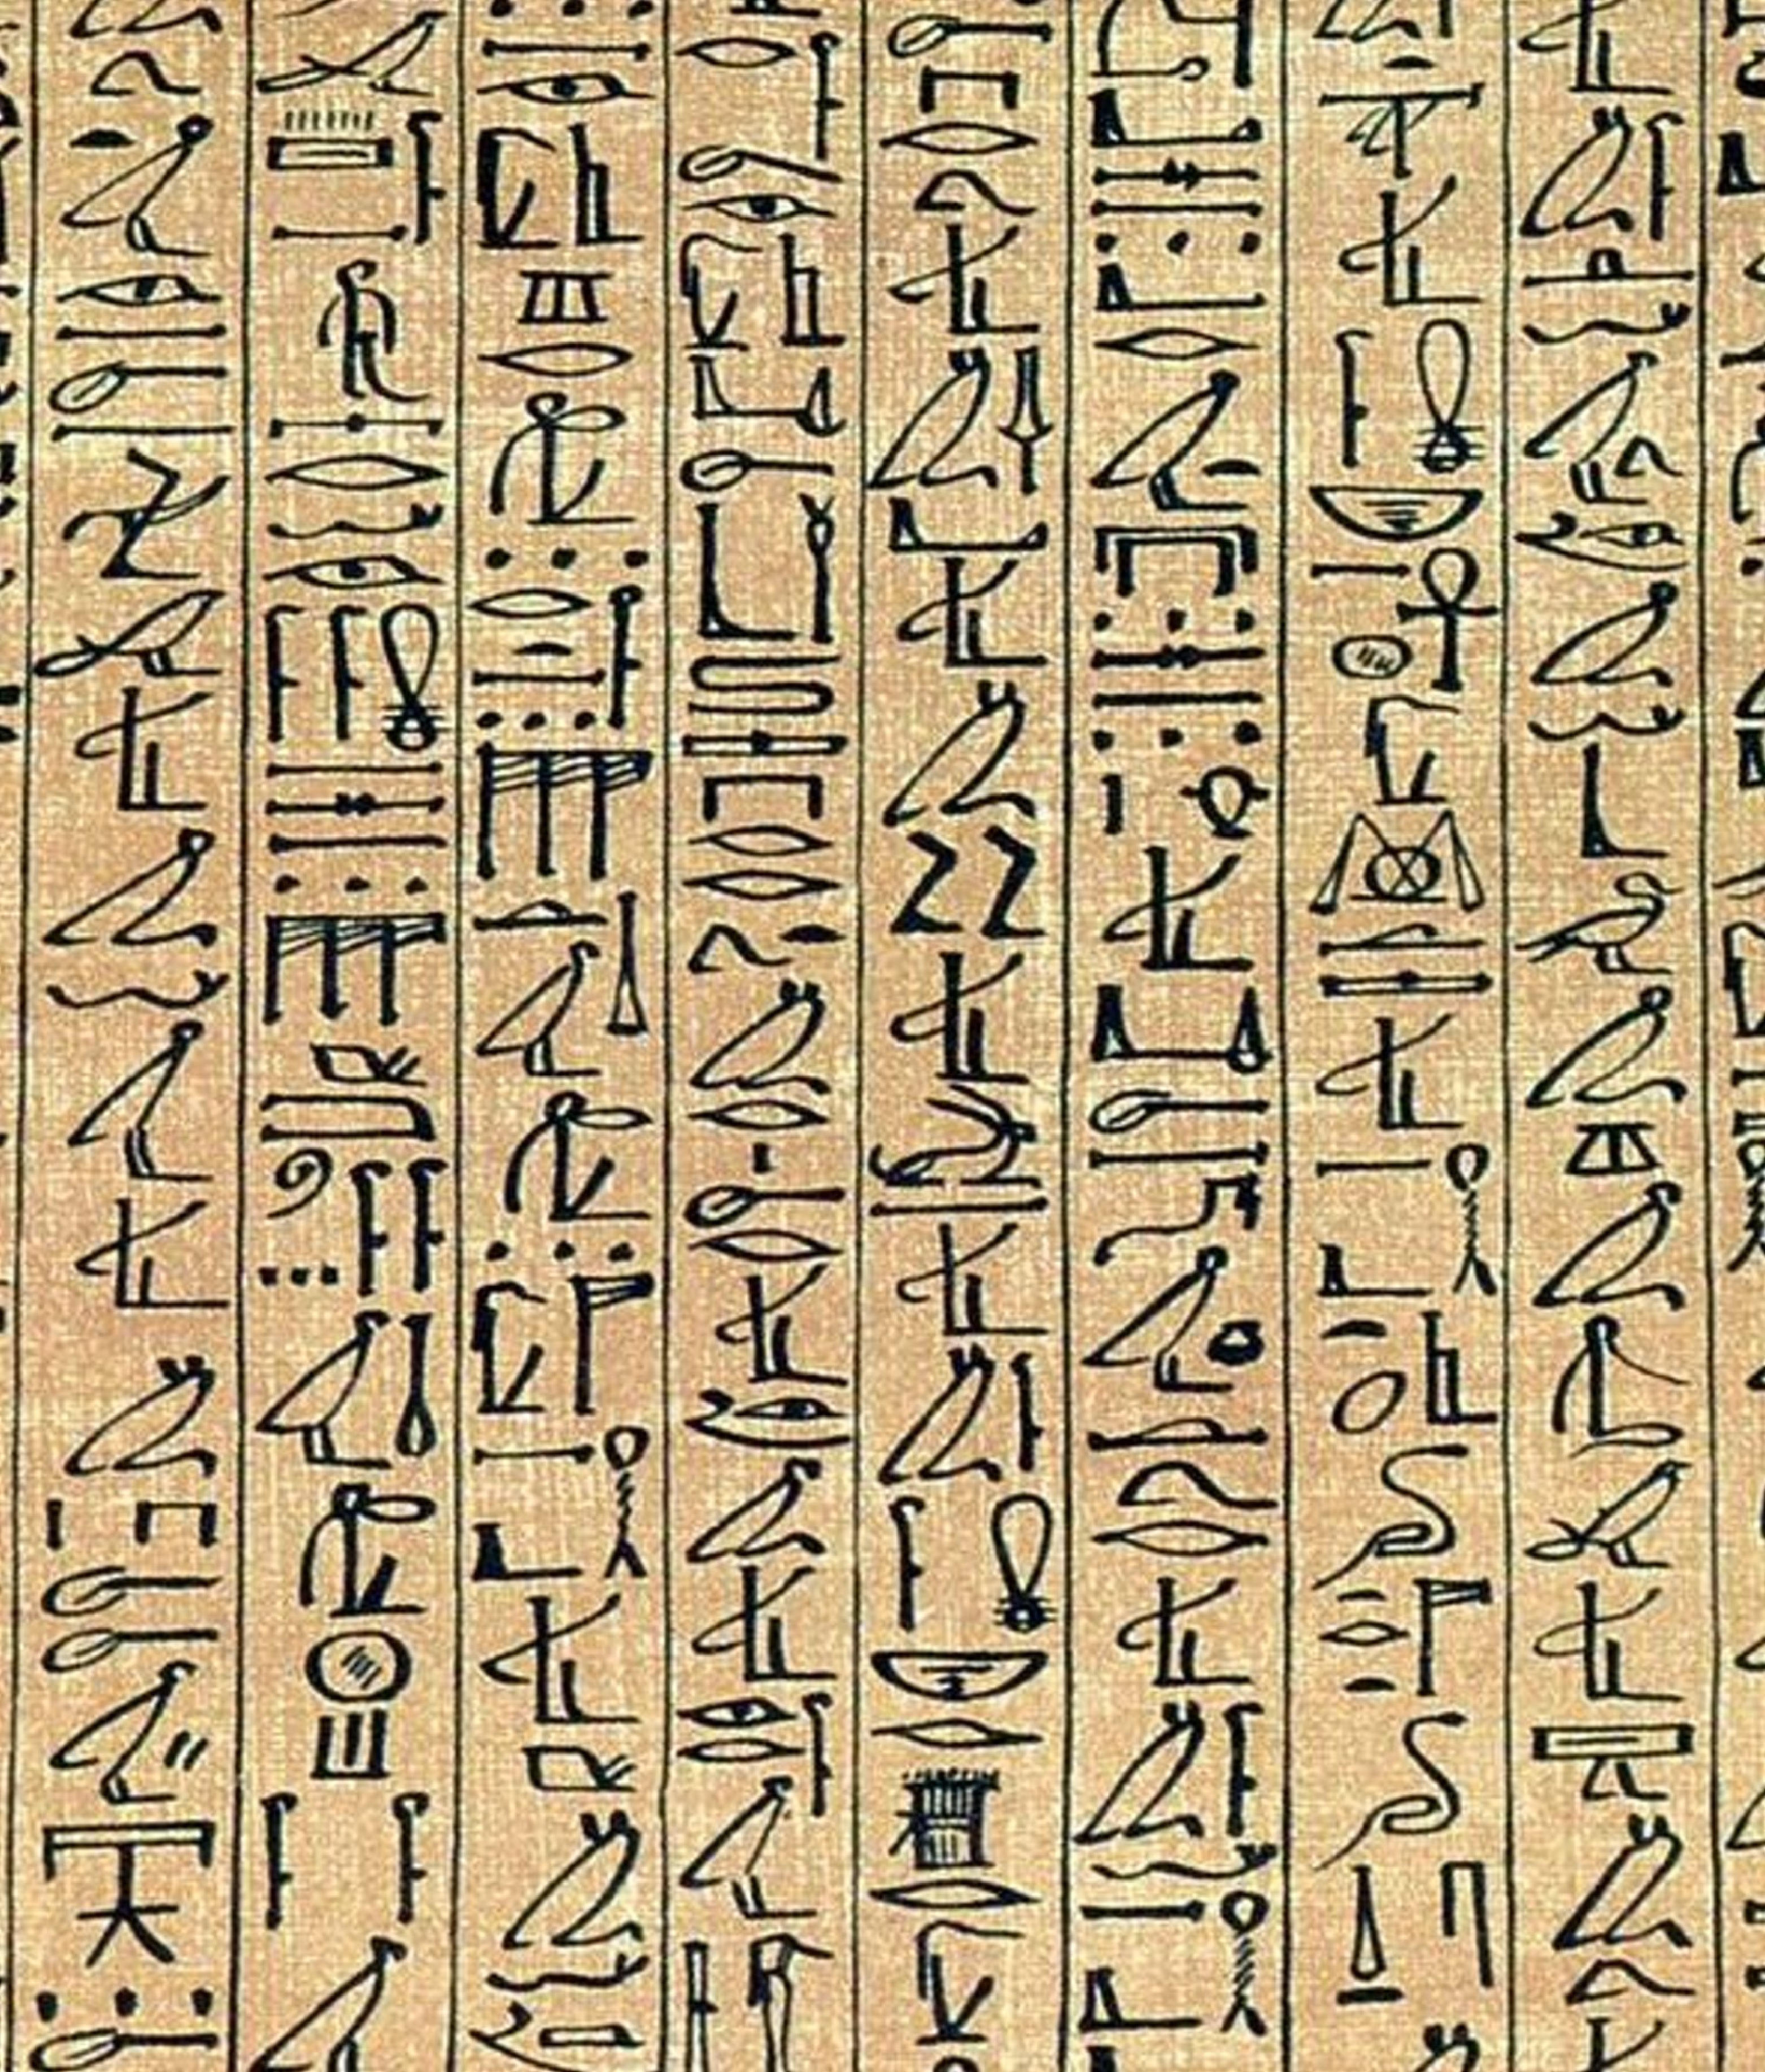
\includegraphics[width=5cm]{figs/egyptian.pdf}
\end{frame}

%------------------------------------------------
\begin{frame}
\frametitle{1450}
\begin{columns}[c] 
\column{30em}
\begin{itemize}
  \justifying
  \item Gutenberg's printing press
\end{itemize}
\end{columns}
\vspace{0.75cm}
\hspace*{4.5cm}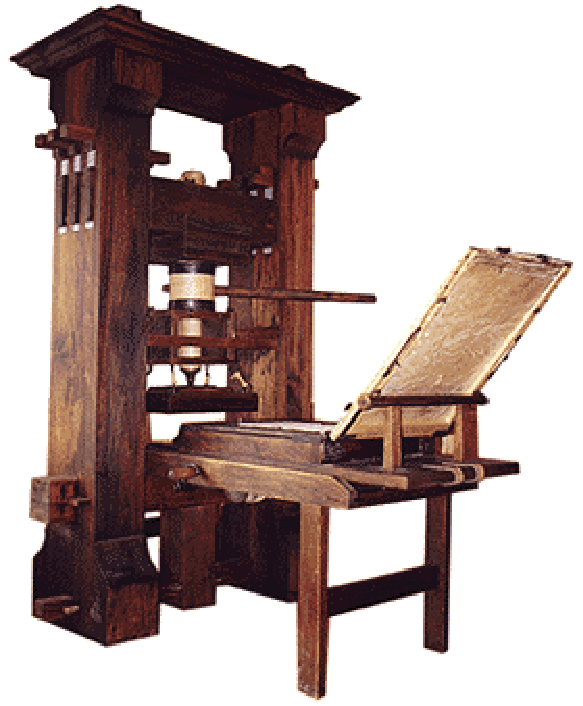
\includegraphics[width=4cm]{figs/gutenberg.pdf}
\end{frame}

%------------------------------------------------
\begin{frame}
\frametitle{1800's - 1940's}
\begin{columns}[c] 
\column{30em}
\begin{itemize}
  \justifying
  \item Punched cards (no fault-tolerance)
  \item Binary data
  \item 1890: US census
  \item 1911: IBM appeared
\end{itemize}
\end{columns}
\vspace{0.5cm}
\begin{columns}[c] 
\column{.4\textwidth}
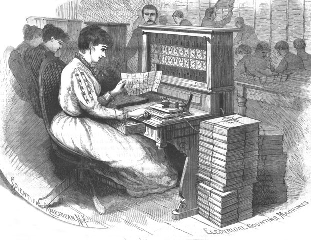
\includegraphics[width=6cm]{figs/punch_card.pdf}
\column{.4\textwidth}
\hspace*{1cm}
\includegraphics[width=4cm]{figs/ibm.pdf}
\end{columns}
\end{frame}

%------------------------------------------------
\begin{frame}
\frametitle{1940's - 1970's}
\begin{columns}[c] 
\column{30em}
\begin{itemize}
  \justifying
  \item Magnetic tapes
  \item Batch transaction processing
  \item File-oriented record processing model (e.g., COBOL)
  \item Hierarchical DBMS (one-to-many)
  \item Network DBMS (many-to-many)
\end{itemize}
\end{columns}
\vspace{0.75cm}
\begin{columns}[c] 
\column{.2\textwidth}
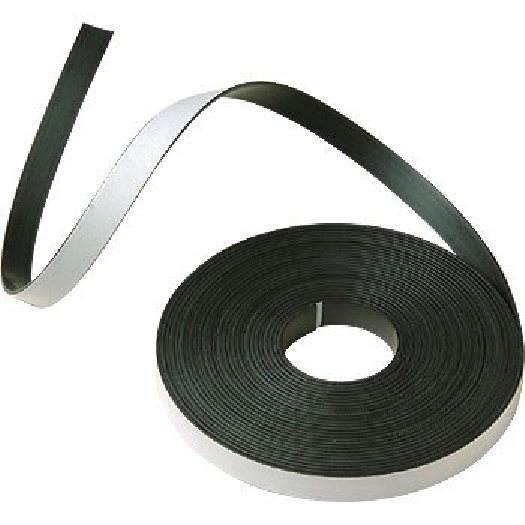
\includegraphics[width=4cm]{figs/tape.pdf}
\column{.4\textwidth}
\hspace*{1cm}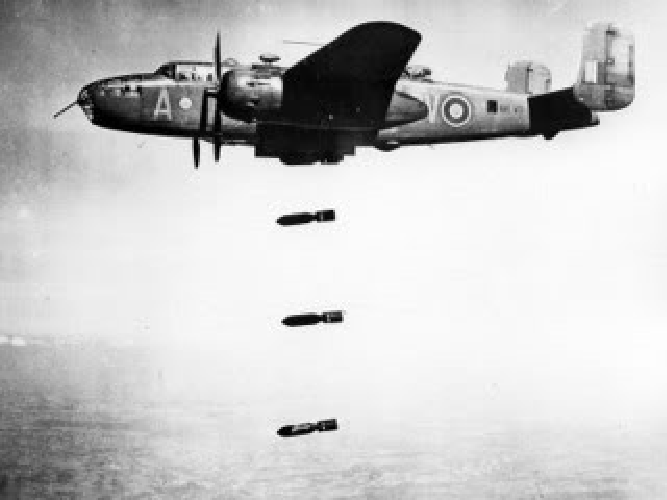
\includegraphics[width=4cm]{figs/bombers.pdf}
\end{columns}
\end{frame}

%------------------------------------------------
\begin{frame}
\frametitle{1980's}
\begin{columns}[c] 
\column{30em}
\begin{itemize}
  \justifying
  \item Relational DBMS (tables) and SQL
  \item ACID
  \item Client-server computing
  \item Parallel processing
\end{itemize}
\end{columns}
\vspace{0.75cm}
\hspace*{2.8cm}
\includegraphics[width=6cm]{figs/acid.pdf}
\end{frame}

%------------------------------------------------
\begin{frame}
\frametitle{1990's - 2000's}
\begin{columns}[c] 
\column{30em}
\begin{itemize}
  \justifying
  \item The Internet...
\end{itemize}
\end{columns}
\vspace{0.75cm}
\hspace*{2.5cm}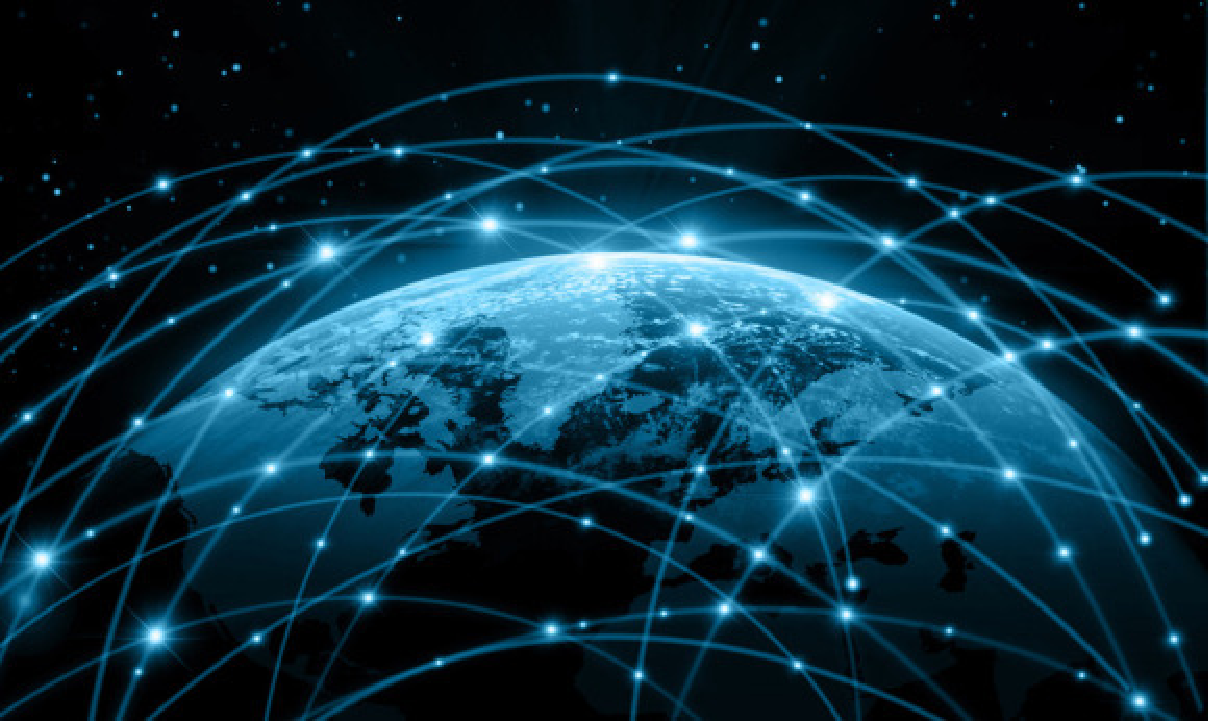
\includegraphics[width=7cm]{figs/internet.pdf}
\end{frame}

%------------------------------------------------
\begin{frame}
\frametitle{2010's}
\begin{columns}[c] 
\column{30em}
\begin{itemize}
  \justifying
  \item NoSQL: BASE instead of ACID
  \item Big Data
\end{itemize}
\end{columns}
\vspace{0.75cm}
\hspace*{3cm}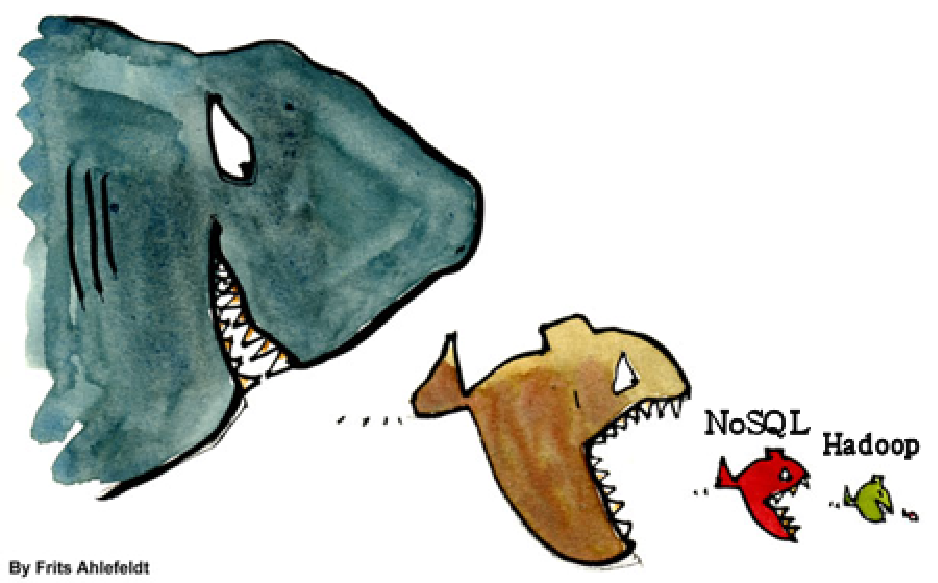
\includegraphics[width=6cm]{figs/nosql.pdf}
\end{frame}

%------------------------------------------------
%\begin{frame}
%\frametitle{too BIG to IGNORE}
%\vspace{2cm}
%\begin{columns}
%\column{30em}
%\begin{block}{}
%\centering
%Everyone talks about it, nobody really knows how to do it, everyone thinks everyone else is doing it, so everyone claims they are doing it.
%\vspace{.1cm}
%\hspace*{9cm}\footnotesize{- Dan Ariely}
%\end{block}
%\end{columns}
%\vspace{.5cm}
%\hspace*{10cm}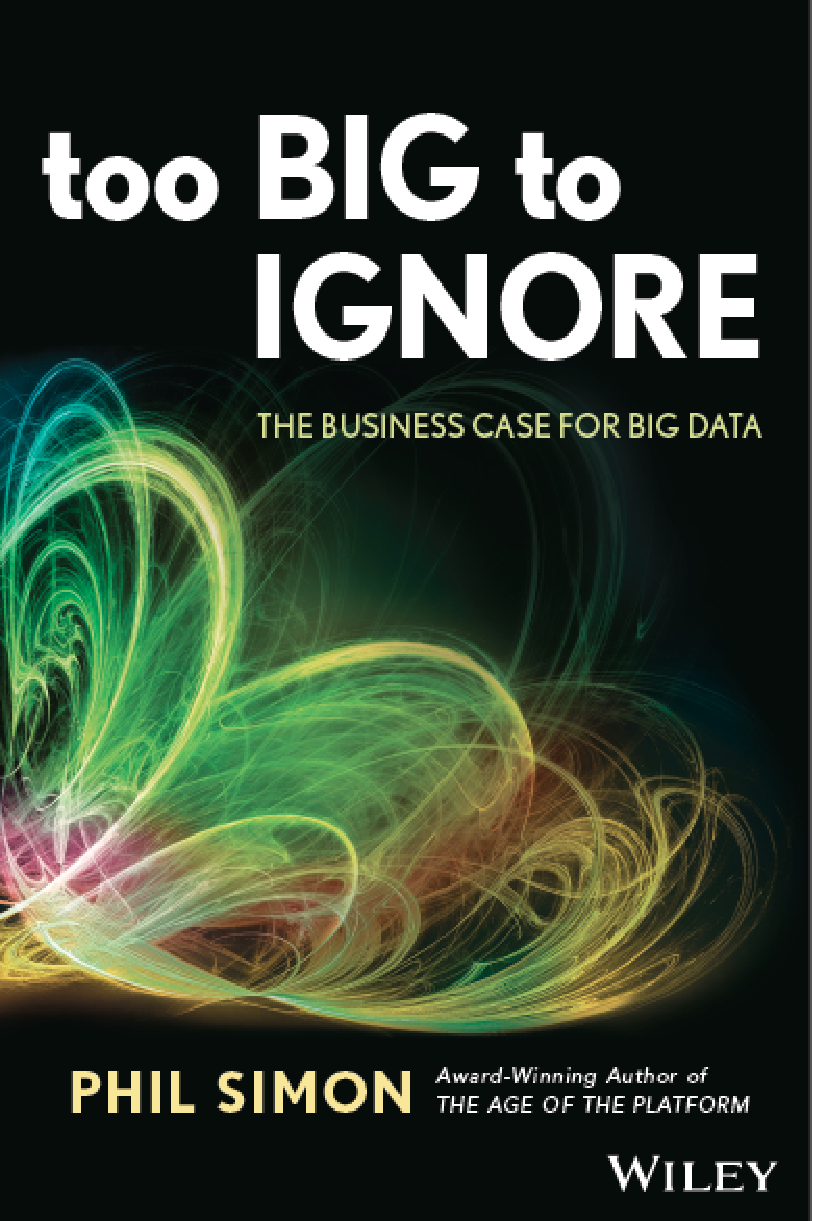
\includegraphics[width=1.5cm]{figs/toobig.pdf}\\
%\end{frame}

%------------------------------------------------
\begin{frame}
\frametitle{Big Data}
\begin{columns}
\column{30em}
\begin{itemize}\itemsep2em
  \justifying
  \item In recent years we have witnessed a \textcolor{Ocean}{dramatic increase} in available data.
  \item For example, the \textcolor{Ocean}{number of web pages} indexed by Google, which were around \textcolor{TextGreen}{one million} in 1998, have exceeded \textcolor{TextGreen}{one trillion} in 2008, and its expansion is accelerated by appearance of the social networks.
\end{itemize}
\end{columns}
\vspace{0.35cm}
\hspace*{8.7cm}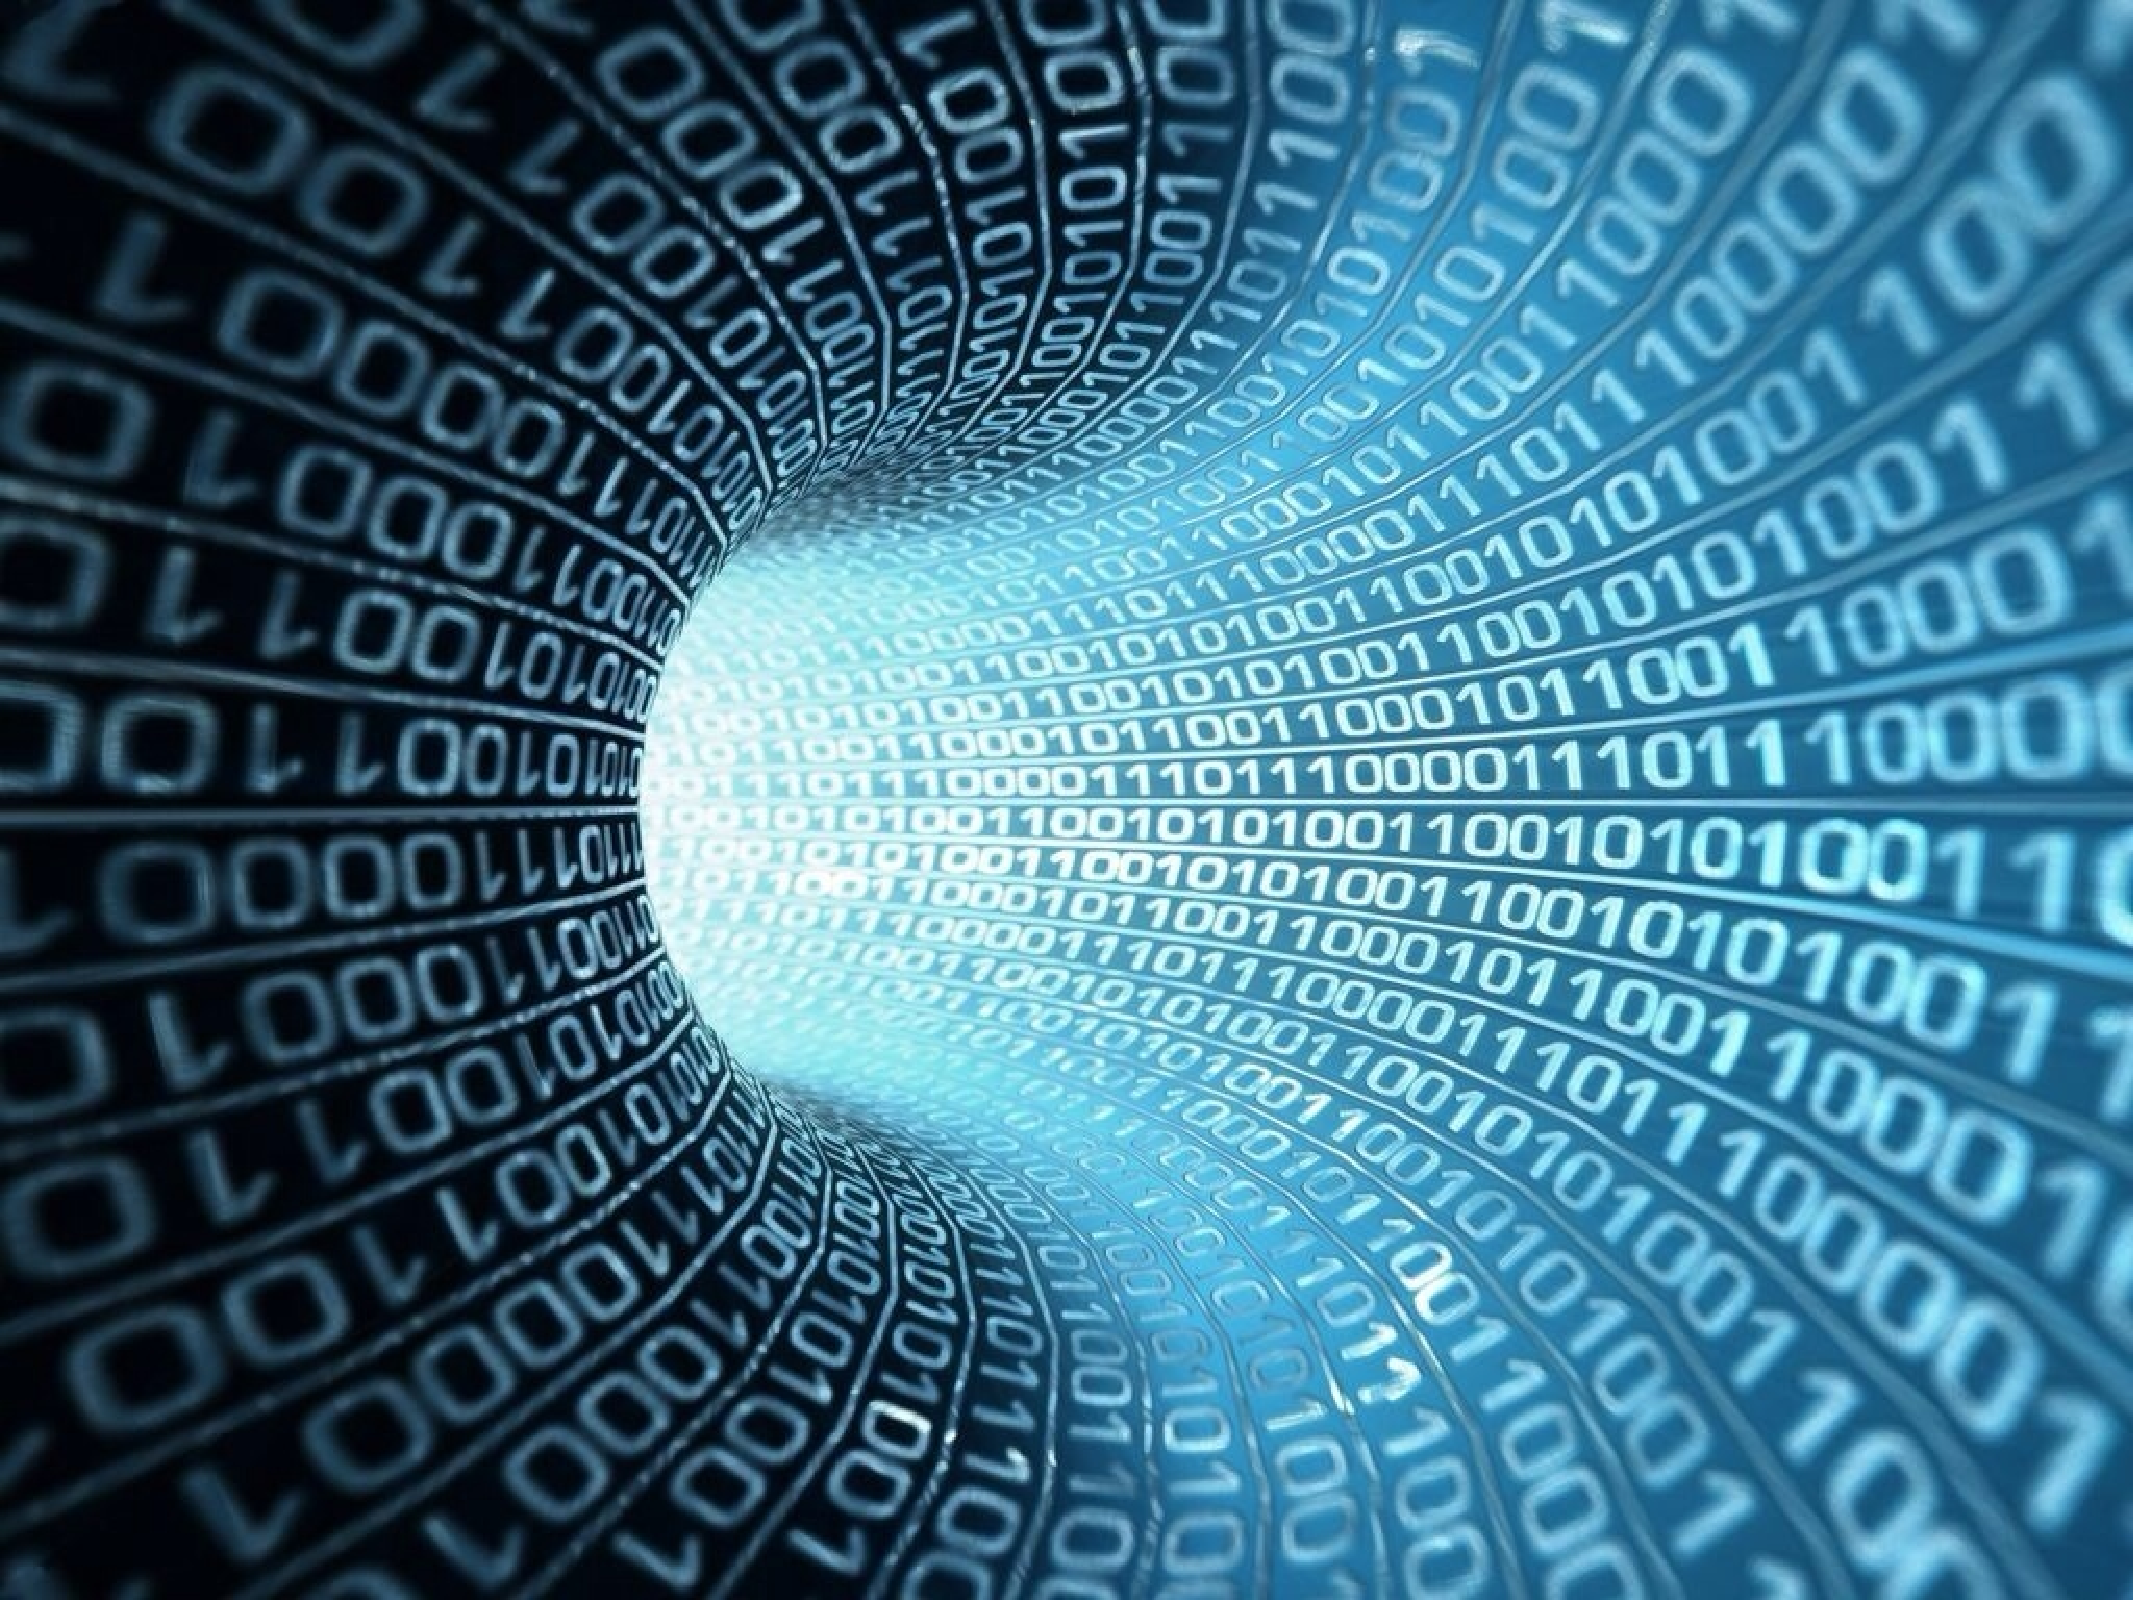
\includegraphics[width=3cm]{figs/zeroone.pdf}
\end{frame}

%------------------------------------------------
\begin{frame}
\frametitle{Big Data Definition}
\begin{columns}[c] 
\column{.65\textwidth}
\begin{itemize}\itemsep2em
  \justifying
  \item \textcolor{darkred}{Big Data} refers to datasets and flows \textcolor{Ocean}{large enough} that has outpaced our capability to \textcolor{TextGreen}{store}, \textcolor{TextGreen}{process}, \textcolor{TextGreen}{analyze}, and \textcolor{TextGreen}{understand}.
\end{itemize}

\column{.25\textwidth}
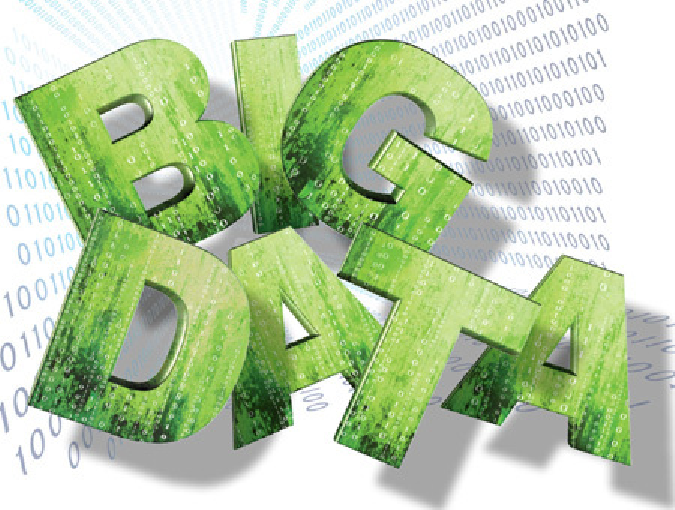
\includegraphics[width=3cm]{figs/big-data.pdf}
\end{columns}
\end{frame}

%------------------------------------------------
\begin{frame}
\frametitle{The Four Dimensions of Big Data}
\begin{columns}[c] 
\column{.6\textwidth}
\begin{itemize}\itemsep1em
  \justifying
  \item \textcolor{Ocean}V\textcolor{darkred}{olume}: data \textcolor{TextGreen}{size}
  \item \textcolor{Ocean}V\textcolor{darkred}{elocity}: data \textcolor{TextGreen}{generation rate}
  \item \textcolor{Ocean}V\textcolor{darkred}{ariety}: data \textcolor{TextGreen}{heterogeneity}
  \item \textcolor{Ocean}V\textcolor{darkred}{eracity}: \textcolor{TextGreen}{uncertainty} of accuracy and \\ authenticity of data
\end{itemize}

\column{.32\textwidth}
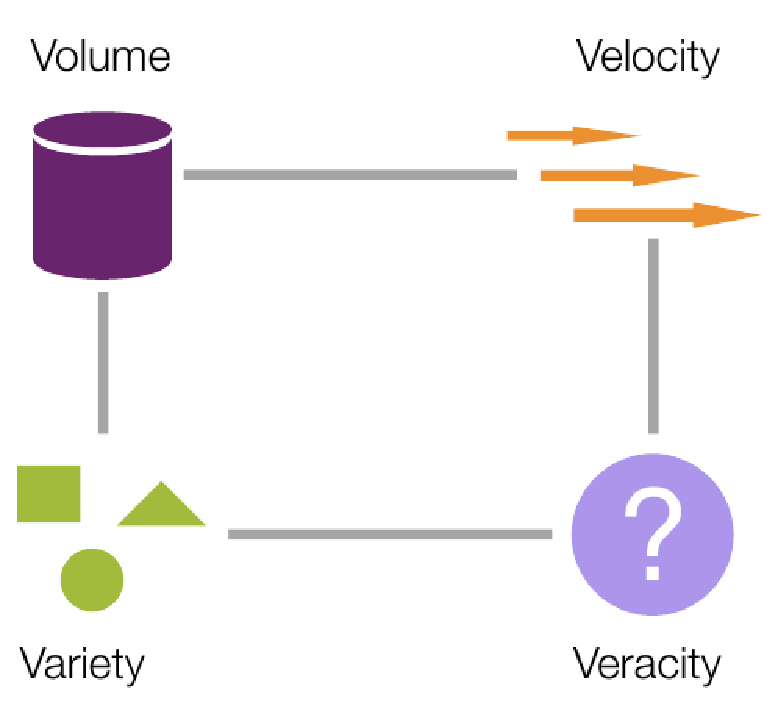
\includegraphics[width=3.5cm]{figs/vs.pdf}
\end{columns}
\end{frame}

%------------------------------------------------
\begin{frame}
\frametitle{Big Data Market Driving Factors}
\begin{columns}[c] 
\column{.4\textwidth}
\begin{itemize}\itemsep2em
  \justifying
  \item Mobile devices
  \item Internet of Things (IoT)
  \item Cloud computing
  \item Open source initiatives
\end{itemize}
\column{.4\textwidth}
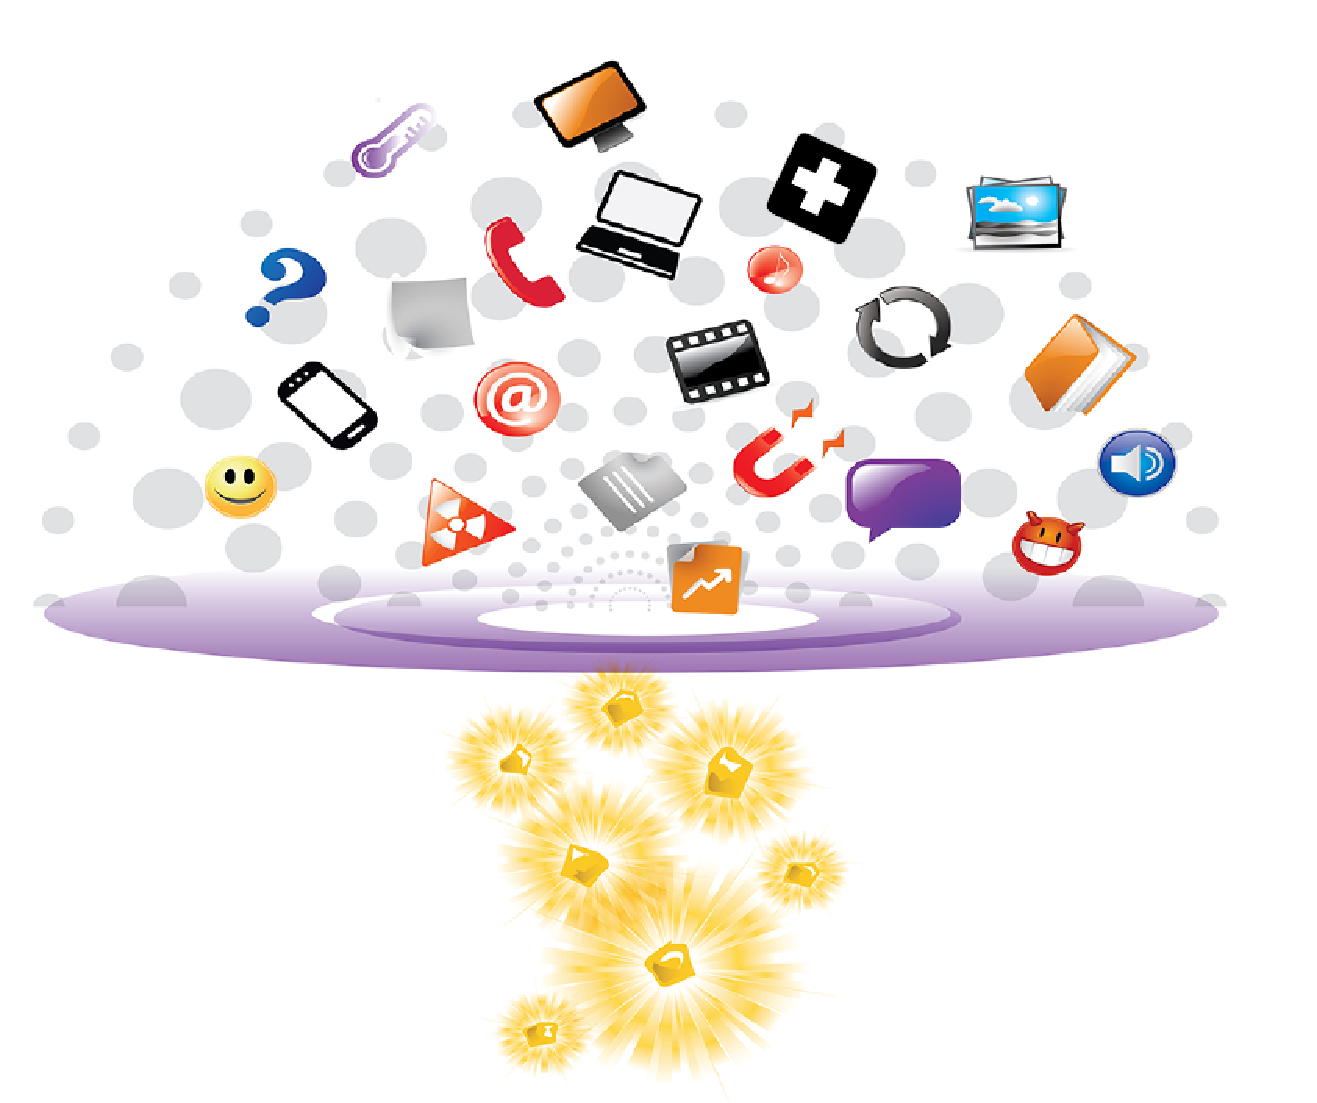
\includegraphics[width=5cm]{figs/driving_factors.pdf}
\end{columns}
\end{frame}

%------------------------------------------------
%\begin{frame}
%\frametitle{Big Data Applications}
%\begin{columns}[c] 
%\column{.55\textwidth}
%\begin{itemize}\itemsep1em
%  \justifying
%  \item Telecommunication and the Internet
%  \item Finance
%  \item Healthcare
%  \item Education
%  \item Transport
%\end{itemize}
%\column{.35\textwidth}
%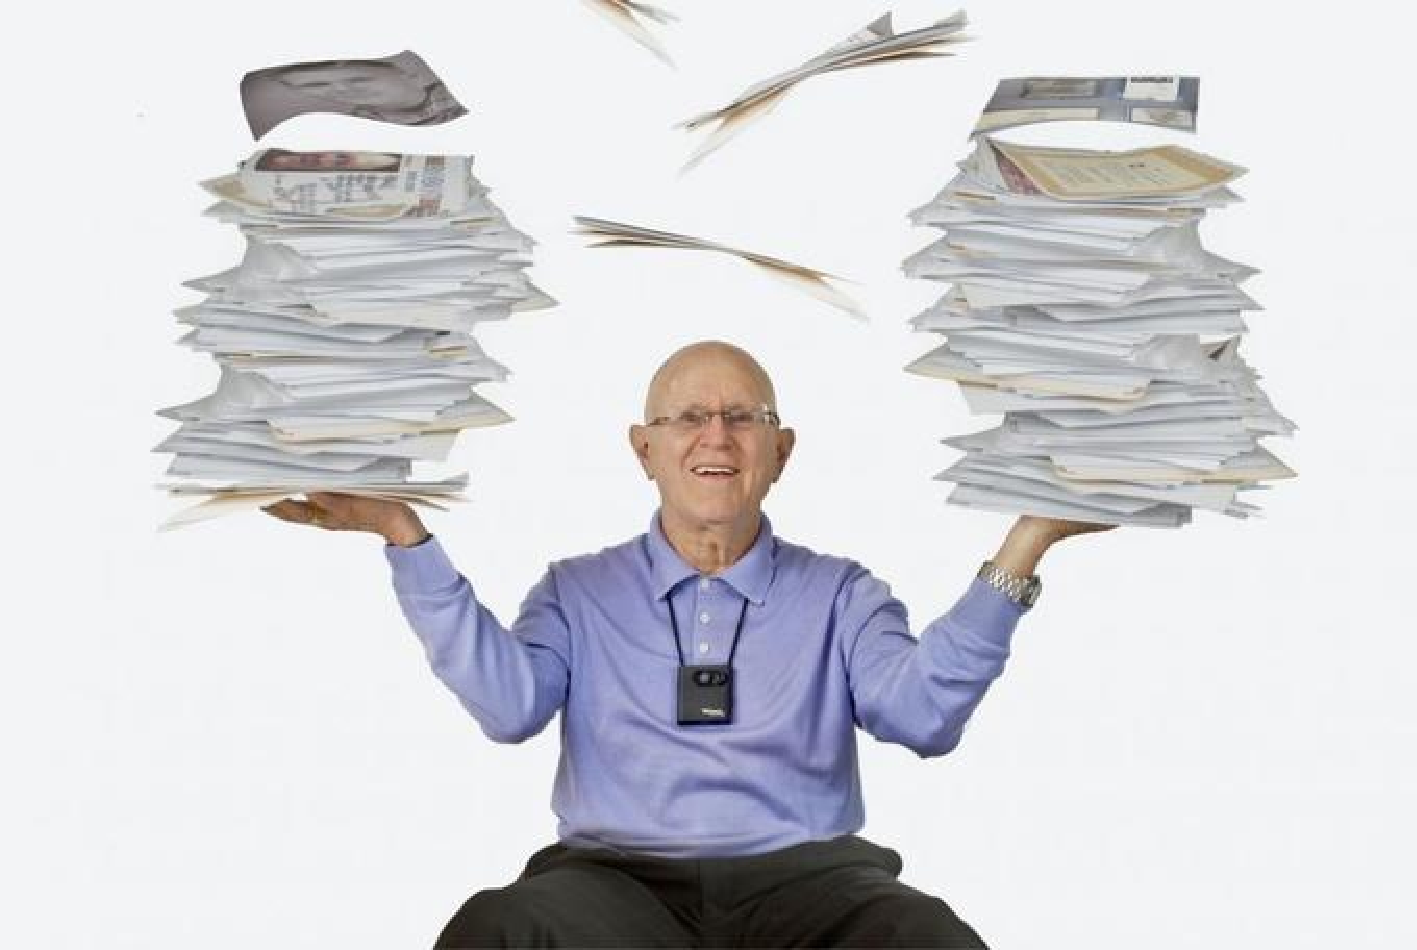
\includegraphics[width=4cm]{figs/applications.pdf}
%\end{columns}
%\end{frame}


%------------------------------------------------
\begin{frame}
\vspace{1cm}
\Huge{\centerline{\usebeamercolor[fg]{title}The Big Data Stack!}}
\end{frame}

%------------------------------------------------
\begin{frame}
\frametitle{Big Data Analytics Stack}
\hspace*{3cm}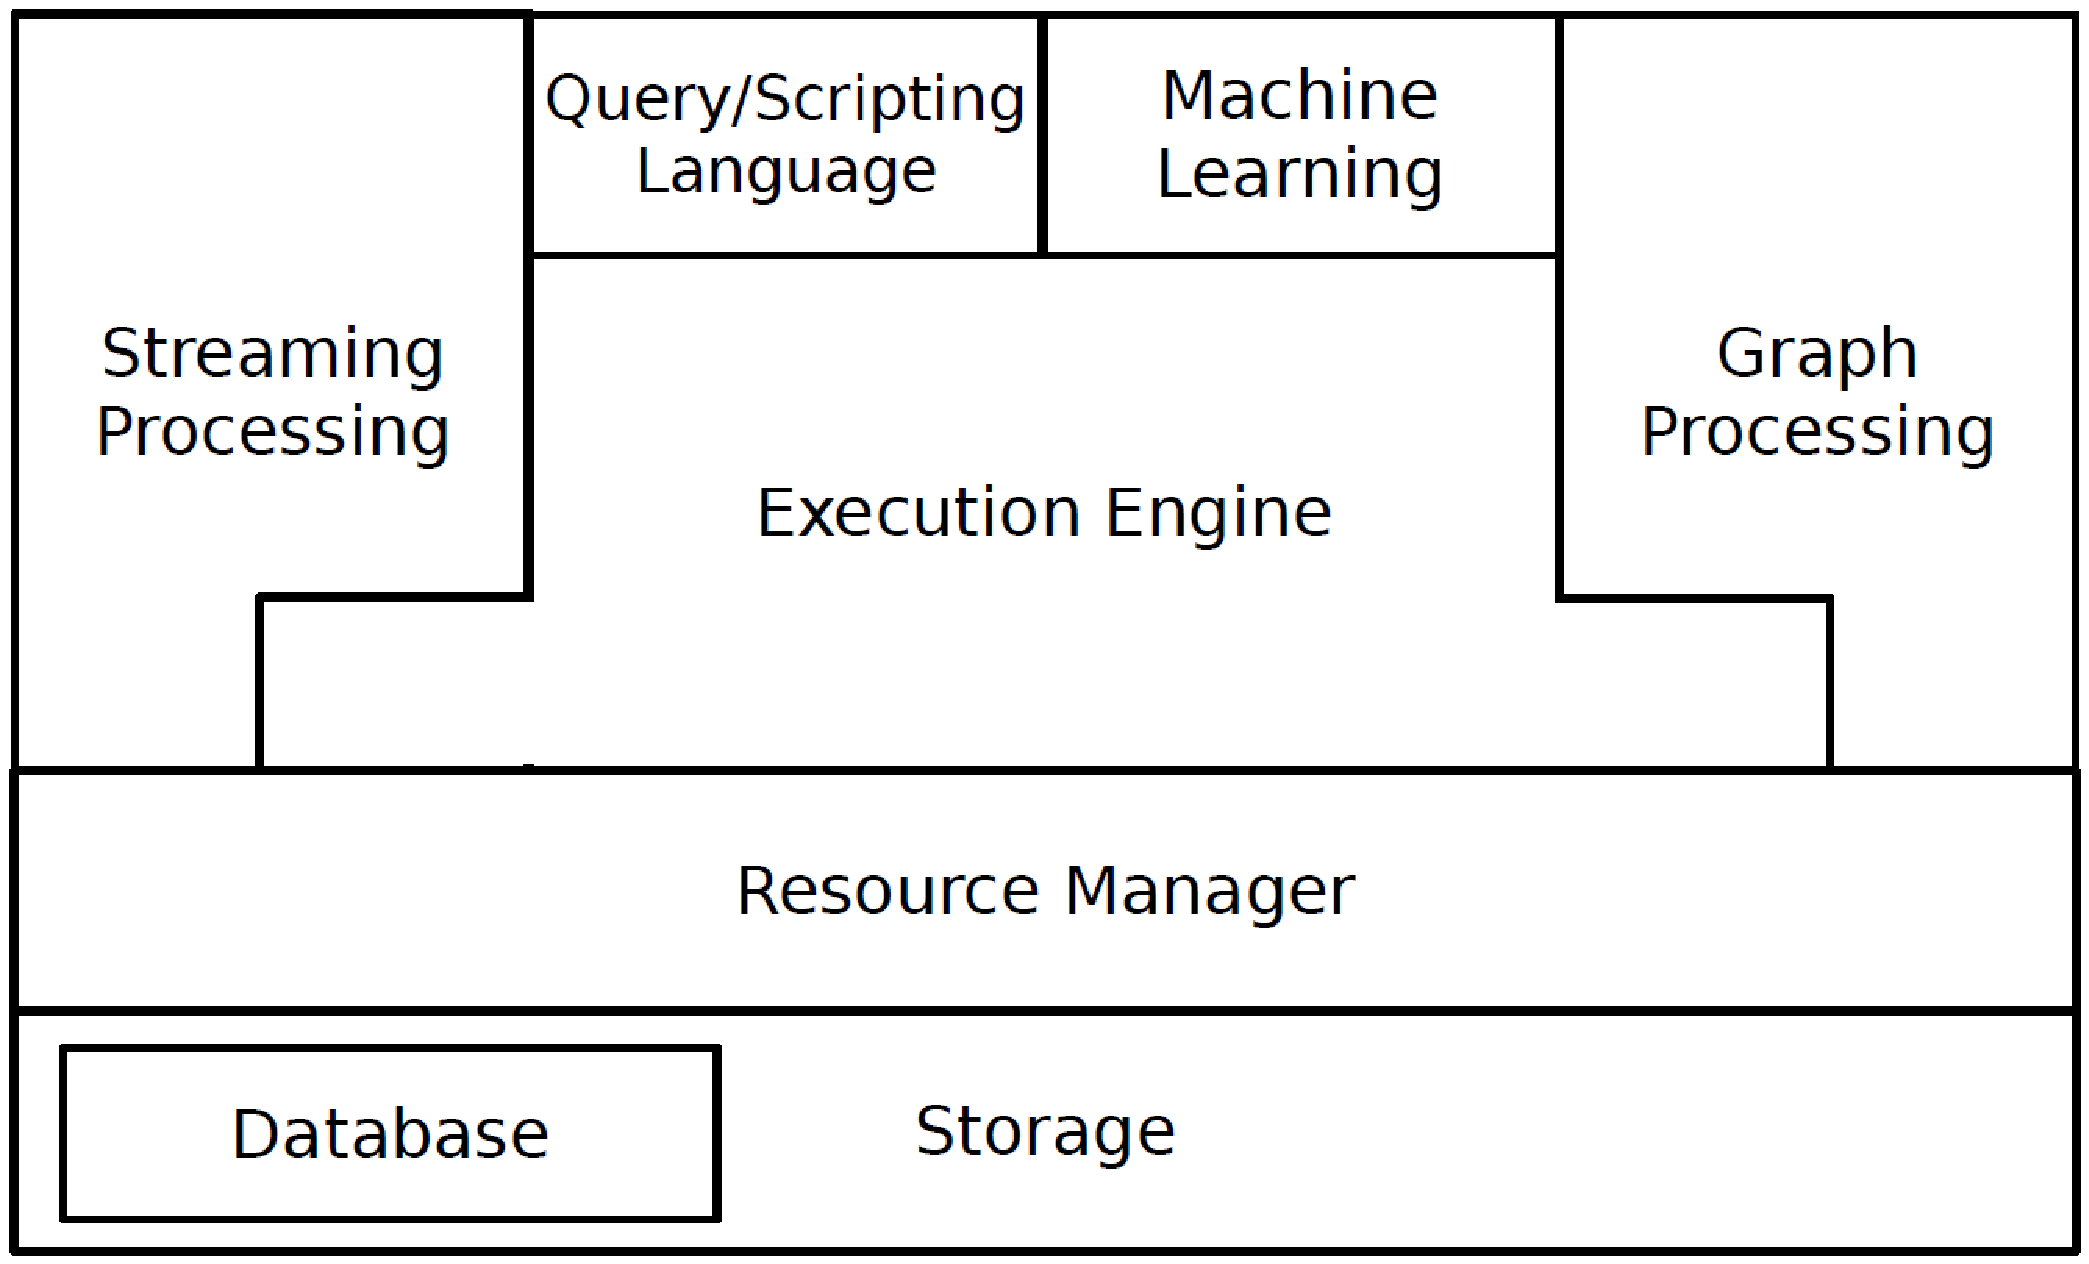
\includegraphics[width=6cm]{figs/stack.pdf}
\end{frame}

%------------------------------------------------
\begin{frame}
\frametitle{Big Data - Storage (Filesystem)}
\begin{columns}
\column{30em}
\begin{itemize}\itemsep1em
  \item Traditional filesystems are not well-designed for large-scale data processing systems. 
  \item \textcolor{TextGreen}{Efficiency} has a higher priority than other features, e.g., directory service. 
  %\item Data tends to be written and read in \textcolor{Ocean}{large batches} at once. 
  \item Massive size of data tends to store it across \textcolor{Ocean}{multiple machines} in a distributed way. 
  \item HDFS, Amazon S3, ...
\end{itemize}
\end{columns}
\vspace{1.2cm}
\hspace*{10cm}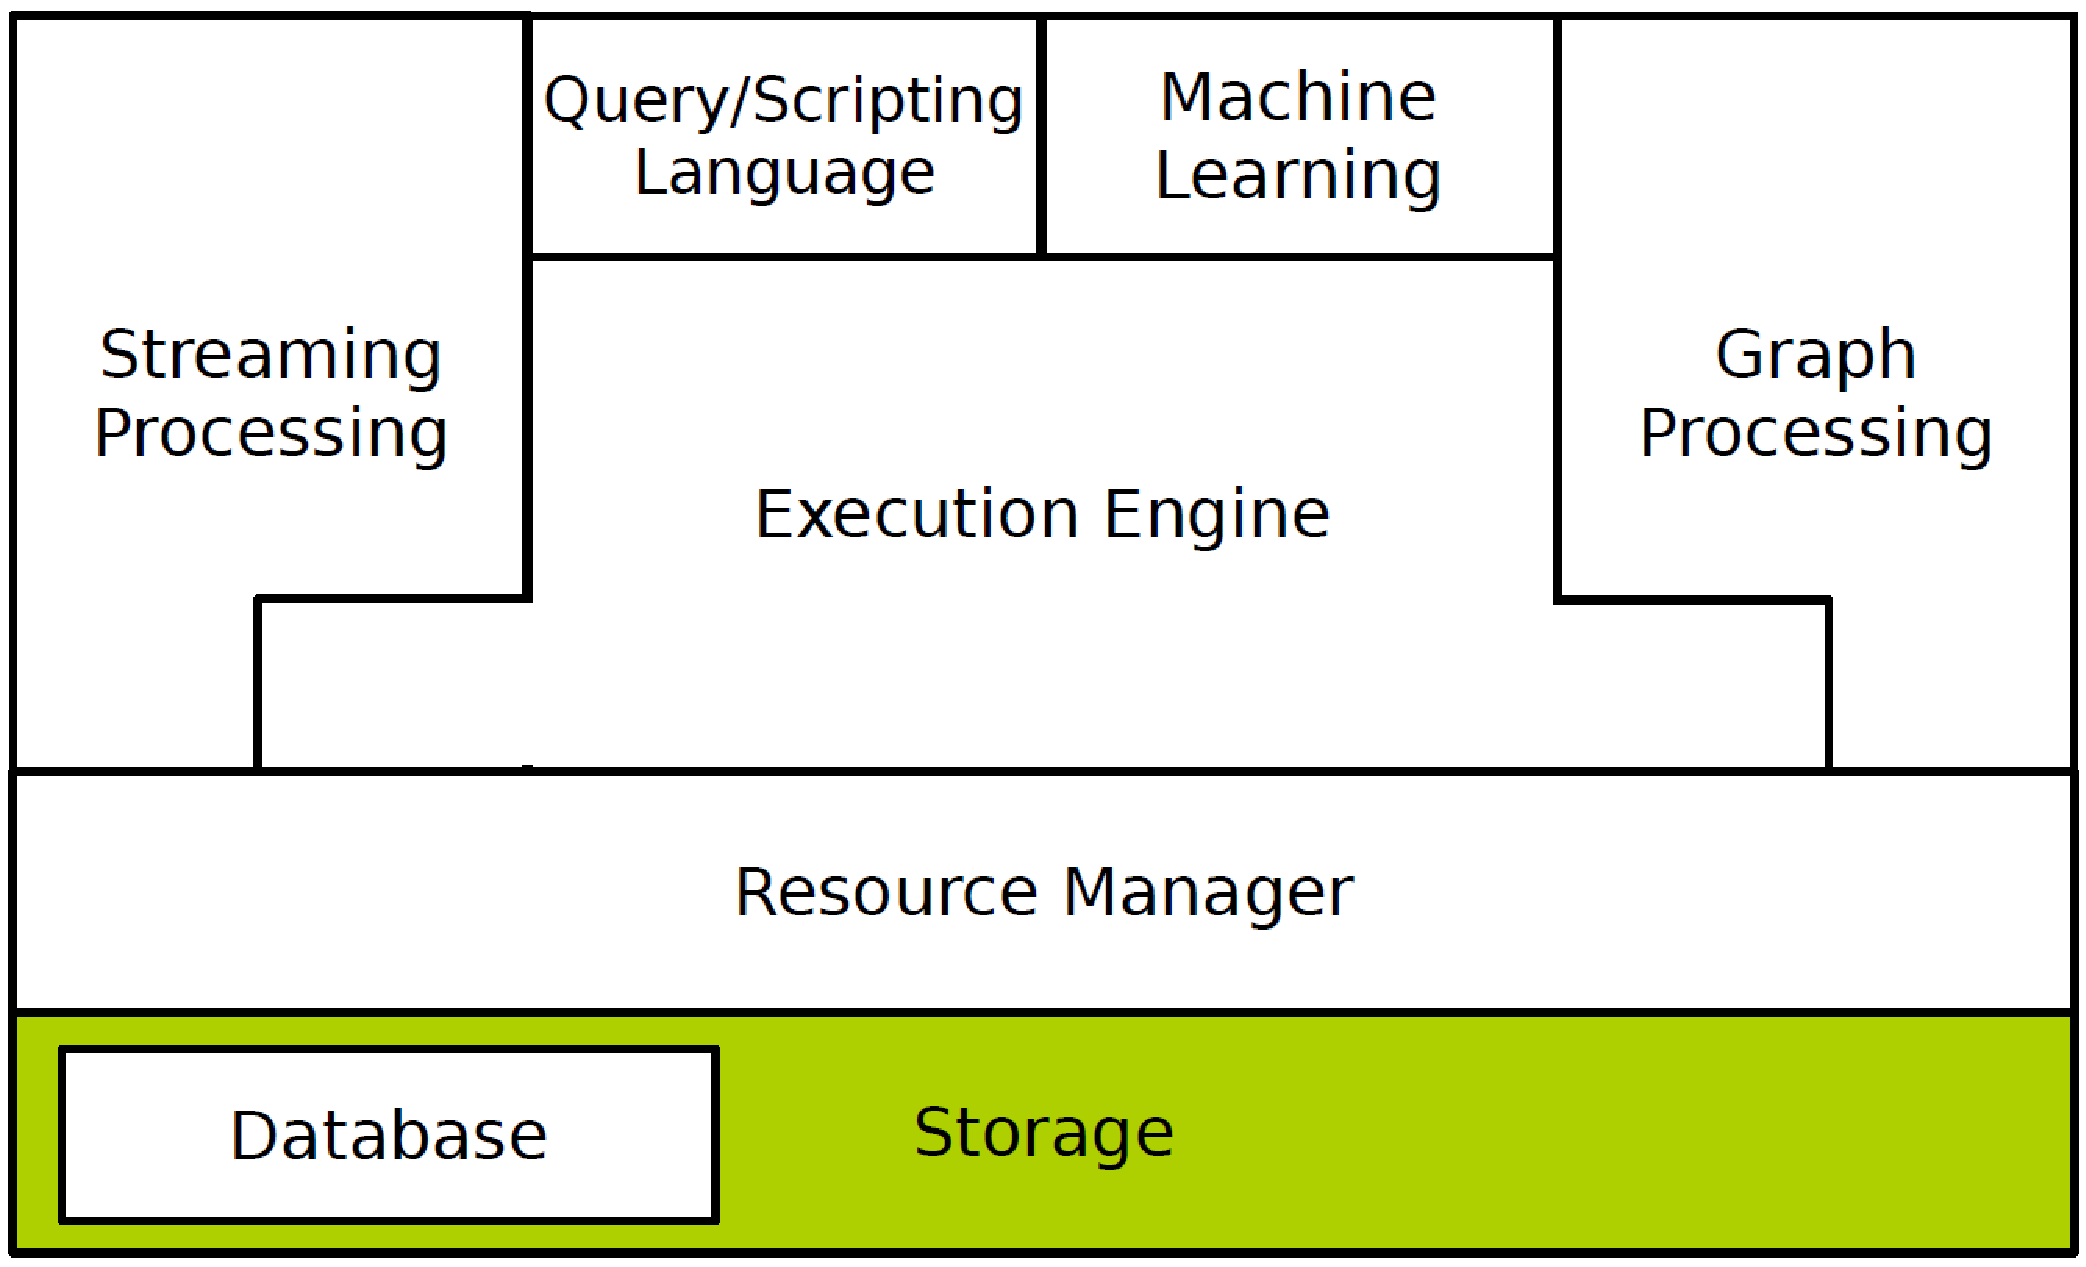
\includegraphics[width=2cm]{figs/stack_storage.pdf}
\end{frame}

%------------------------------------------------
\begin{frame}
\frametitle{Big Data - Database}
\begin{columns}
\column{30em}
\begin{itemize}\itemsep1em
  \justifying
  \item Relational Databases Management Systems \textcolor{Ocean}{(RDMS)} were \textcolor{TextGreen}{not} designed to be distributed.
  \item \textcolor{darkred}{NoSQL} databases \textcolor{Ocean}{relax} one or more of the \textcolor{Ocean}{ACID} properties: \textcolor{TextGreen}{BASE}
  \item Different data models: \textcolor{Ocean}{key/value}, \textcolor{Ocean}{column-family}, \textcolor{Ocean}{graph}, \textcolor{Ocean}{document}.
  \item Dynamo, Scalaris, BigTable, Hbase, Cassandra, MongoDB, Voldemort, Riak, Neo4J, ...
\end{itemize}
\end{columns}
\vspace{1.83cm}
\hspace*{10cm}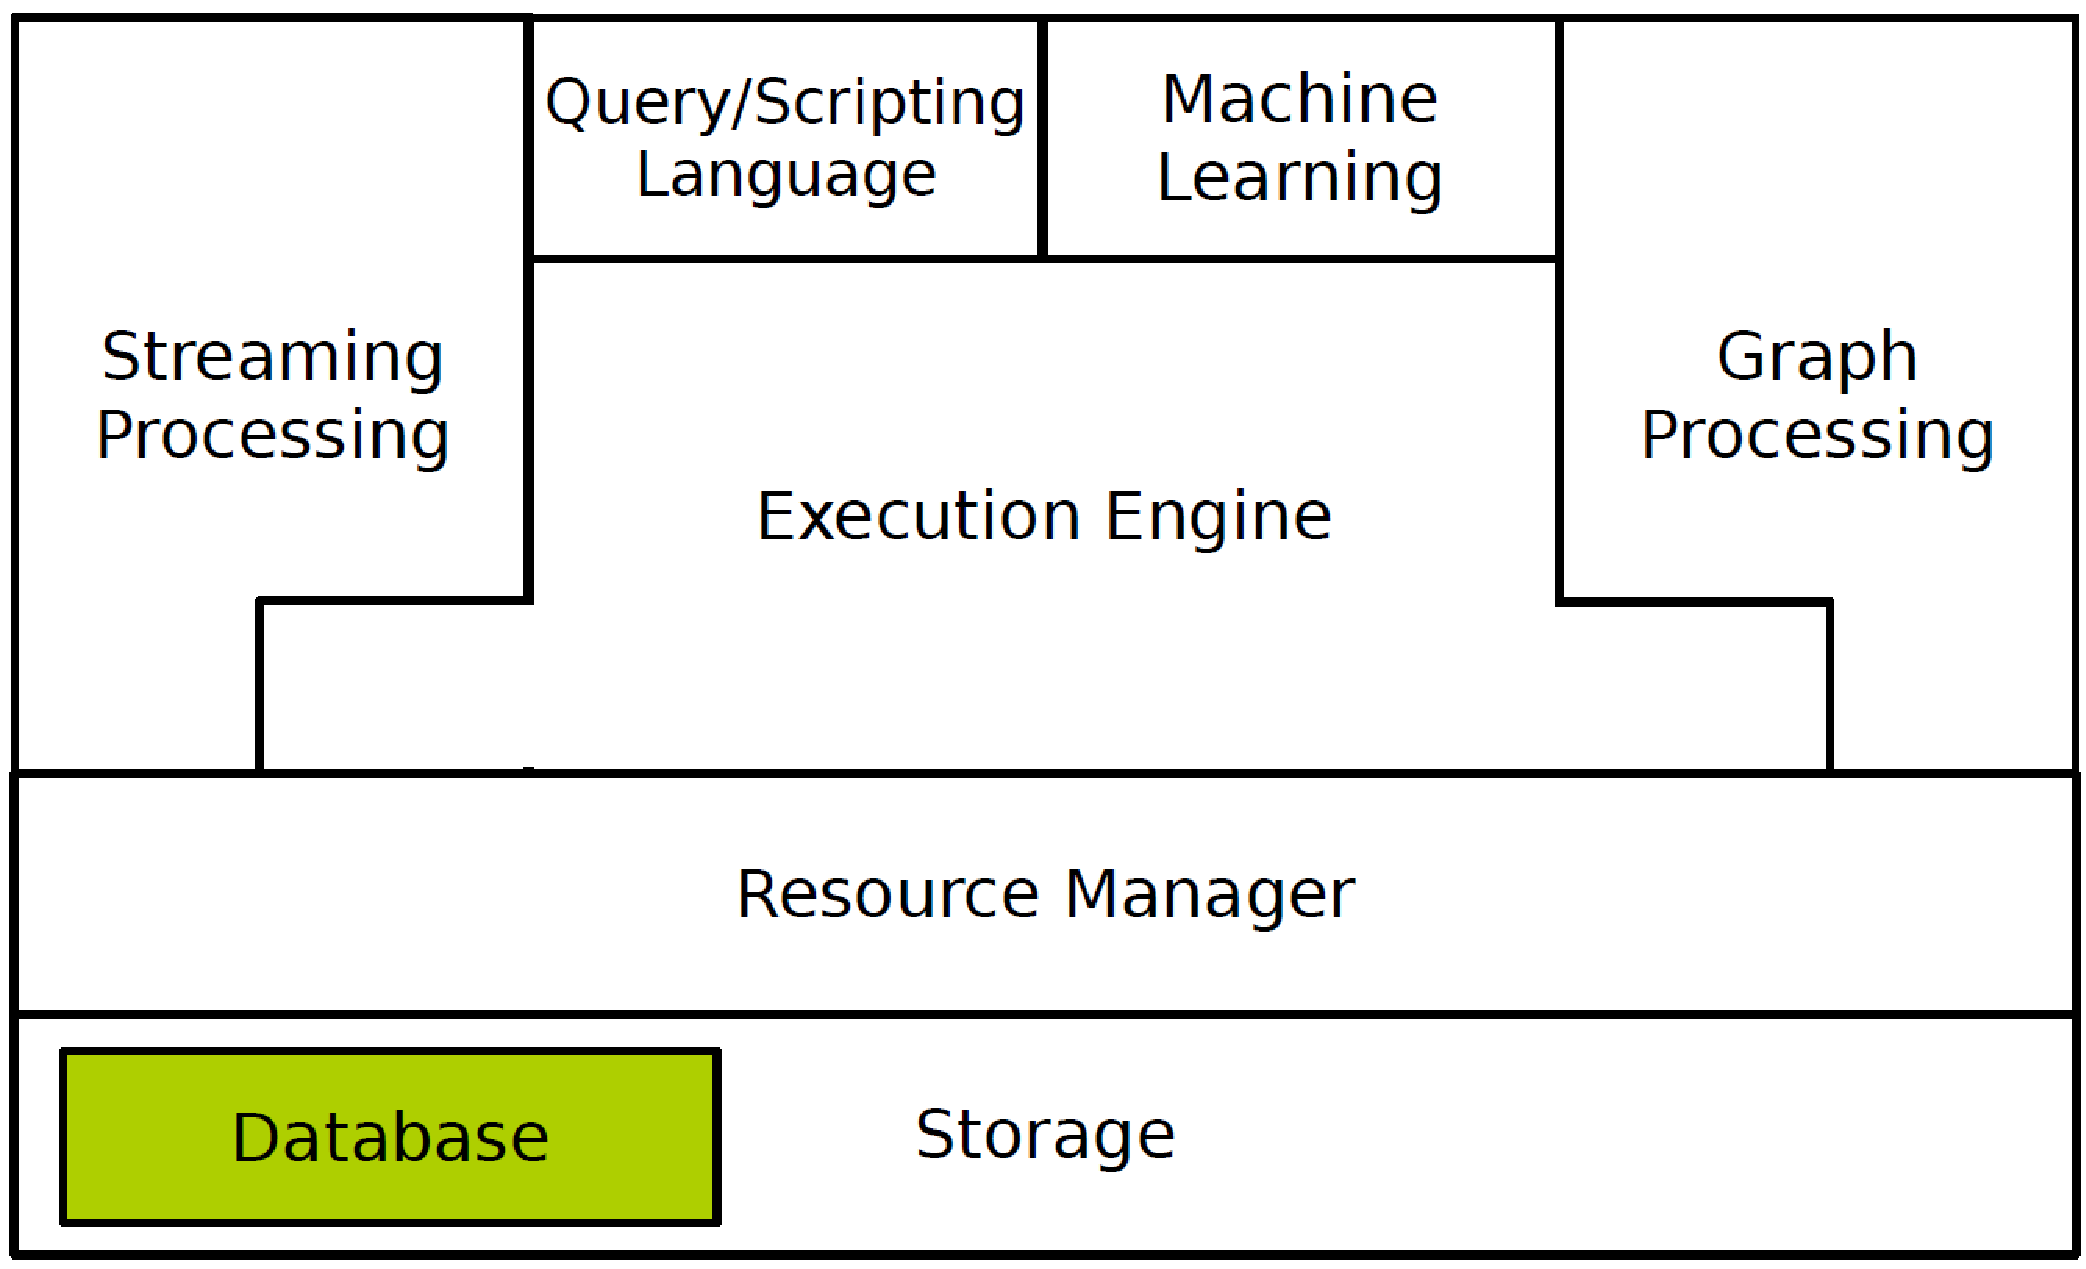
\includegraphics[width=2cm]{figs/stack_database.pdf}
\end{frame}

%------------------------------------------------
\begin{frame}
\frametitle{Big Data - Resource Management}
\begin{columns}
\column{30em}
\begin{itemize}\itemsep1em
  \justifying
  \item Different frameworks require different \textcolor{Ocean}{computing resources}.
  \item Large organizations need the ability to \textcolor{Ocean}{share data and resources} between multiple frameworks. 
  \item \textcolor{darkred}{Resource management} share resources in a cluster between \textcolor{Ocean}{multiple frameworks} while providing resource \textcolor{TextGreen}{isolation}.
  \item Mesos, YARN, Quincy, ...
\end{itemize}
\end{columns}
\vspace{1.8cm}
\hspace*{10cm}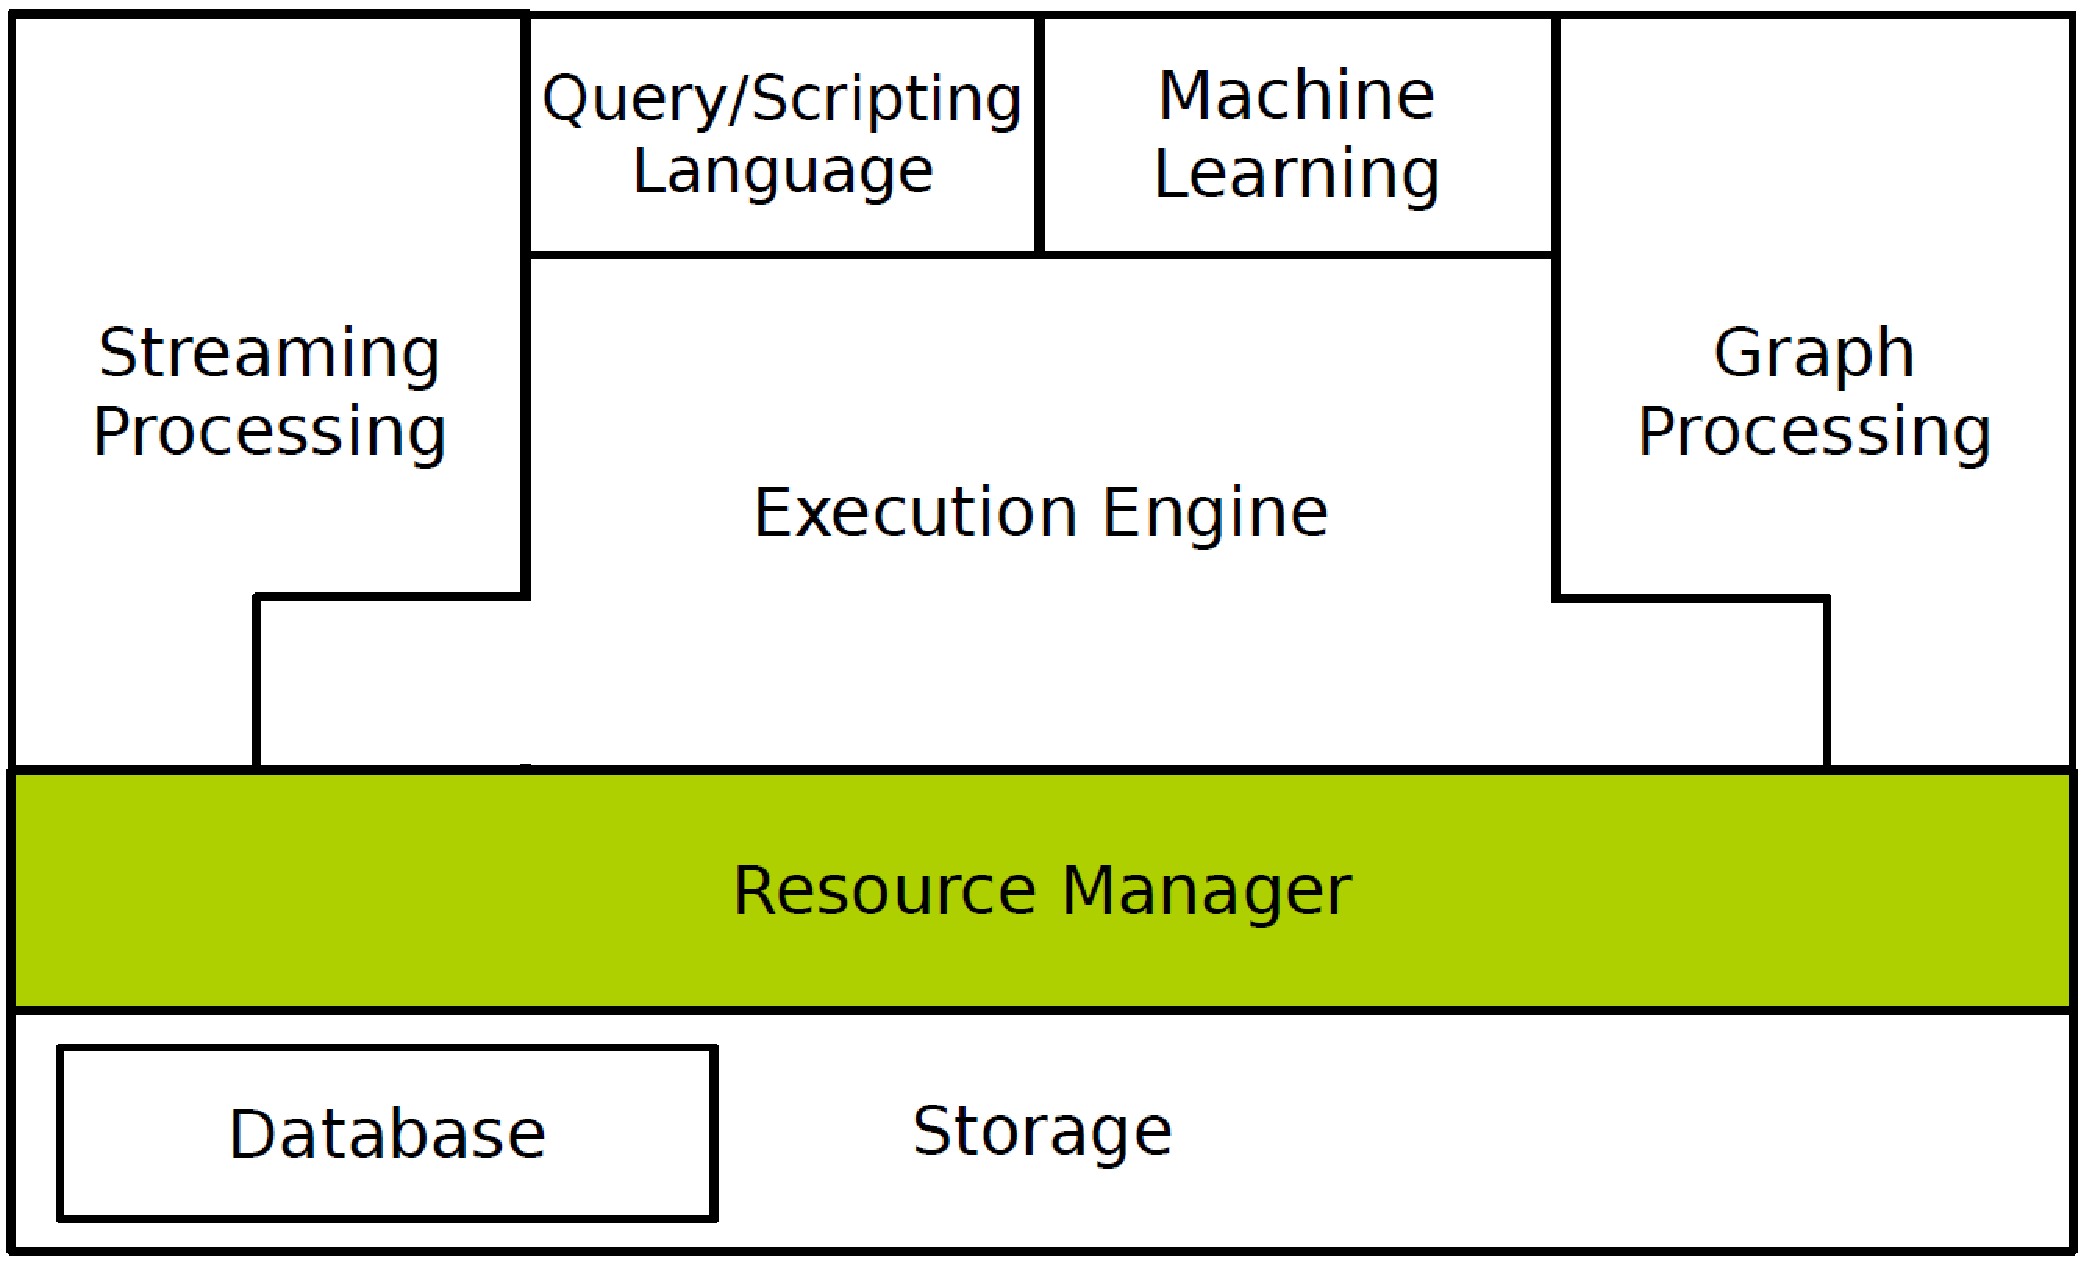
\includegraphics[width=2cm]{figs/stack_job.pdf}
\end{frame}

%------------------------------------------------
\begin{frame}
\frametitle{Big Data - Execution Engine}
\begin{columns}
\column{30em}
\begin{itemize}\itemsep1em
  \justifying
  \item \textcolor{Ocean}{Scalable} and \textcolor{Ocean}{fault tolerance} parallel data processing on clusters of unreliable machines.
  %\item \textcolor{darkred}{Fine-grained} scheduling model is desirable, such that computations are operated on the \textcolor{Ocean}{same node} with the data needed: \textcolor{TextGreen}{lowering the cost}.
  \item Data-parallel \textcolor{Ocean}{programming model} for clusters of commodity machines.
  \item MapReduce, Spark, Stratosphere, Dryad, Hyracks, ...
\end{itemize}
\end{columns}
\vspace{2.55cm}
\hspace*{10cm}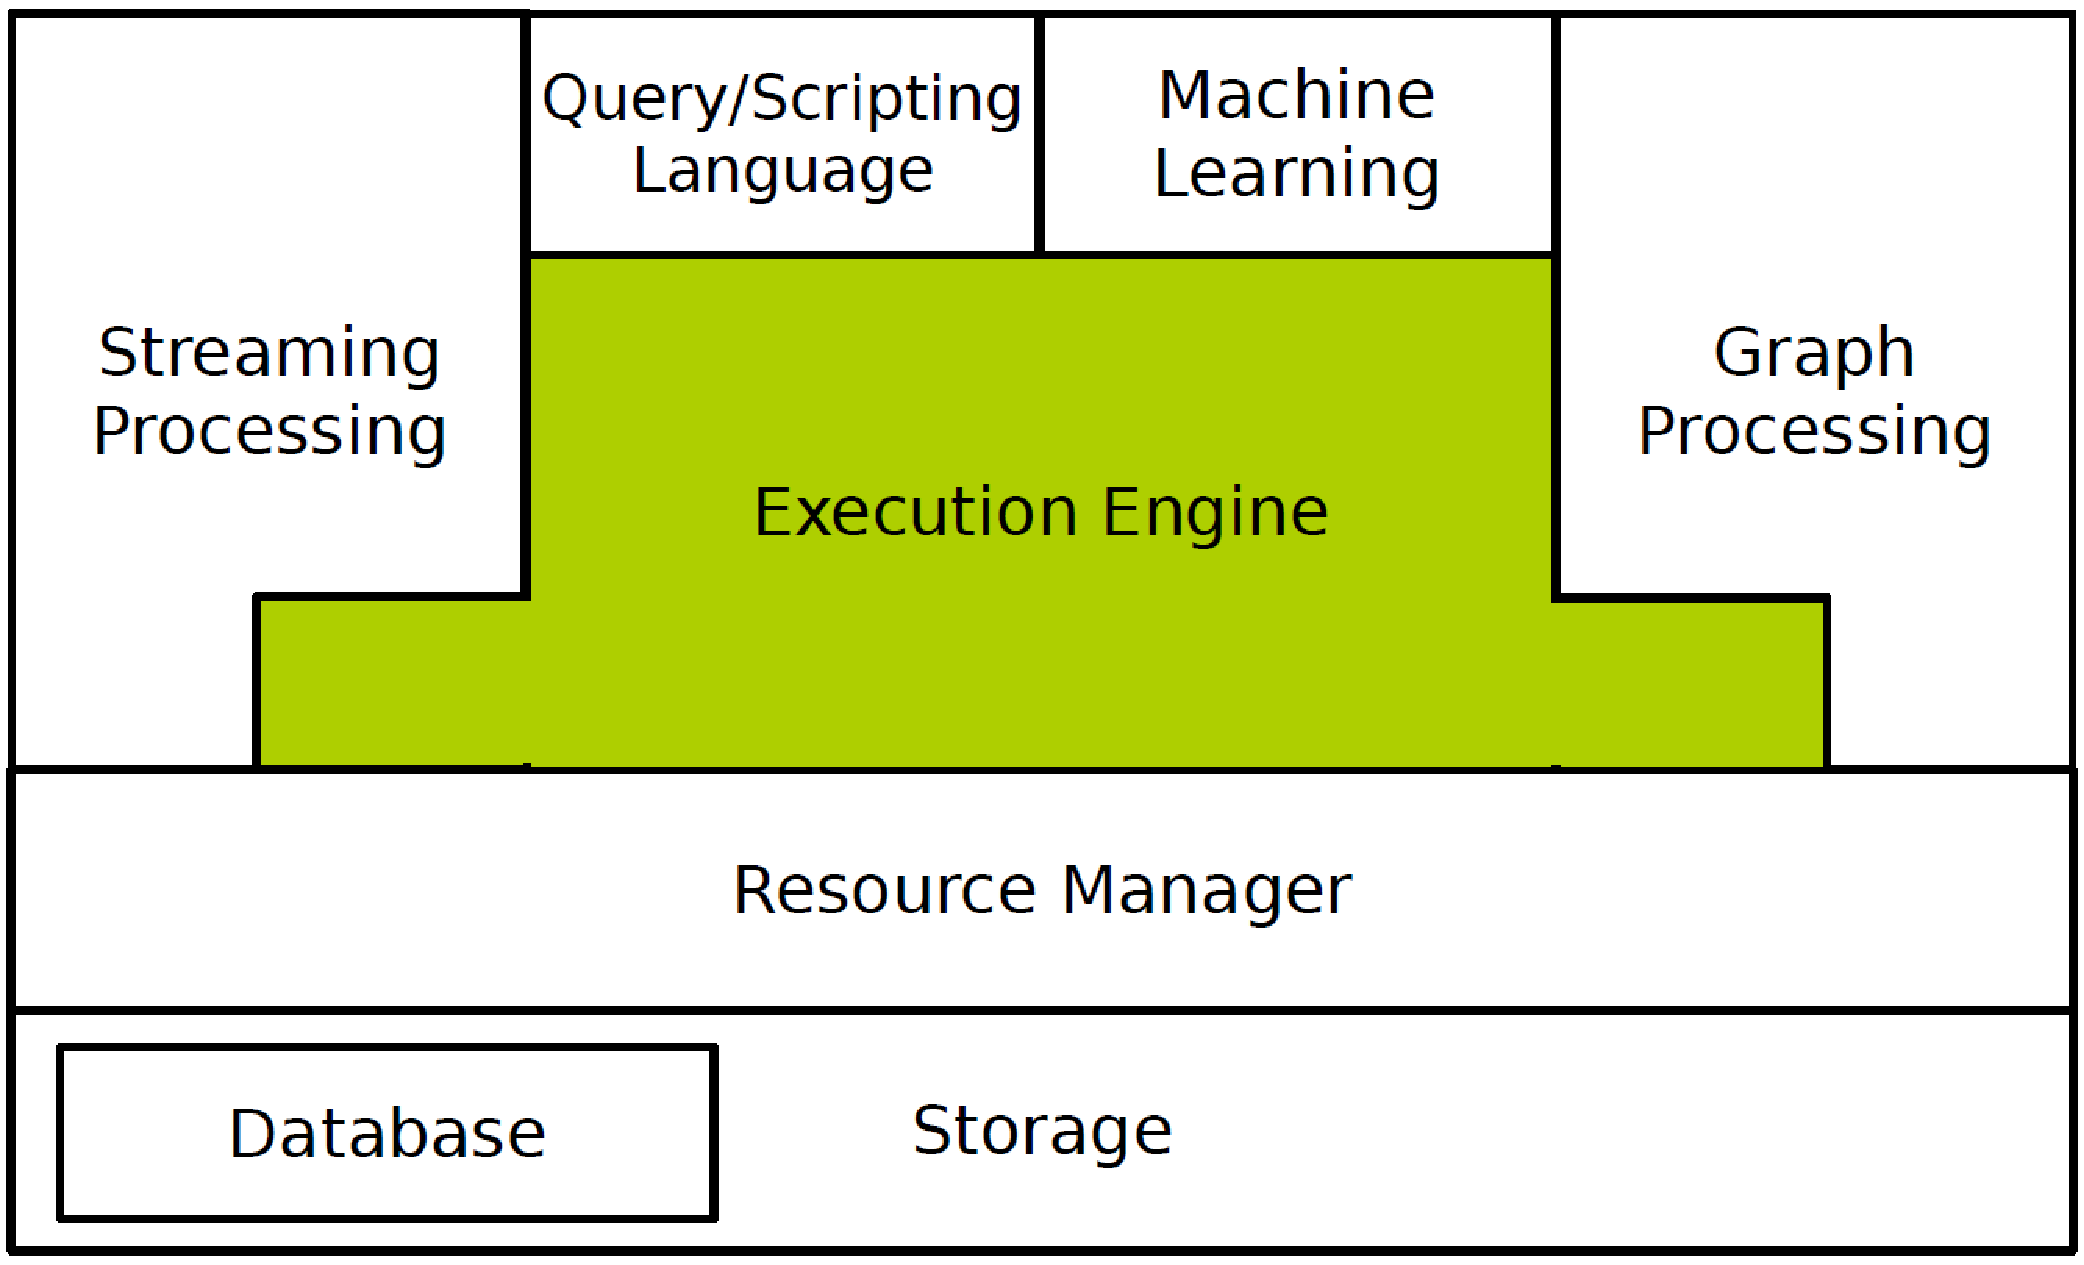
\includegraphics[width=2cm]{figs/stack_execution.pdf}
\end{frame}

%------------------------------------------------
\begin{frame}
\frametitle{Big Data - Query/Scripting Language}
\begin{columns}
\column{30em}
\begin{itemize}\itemsep1em
  \justifying
  \item \textcolor{Ocean}{Low-level} programming of execution engines, e.g., MapReduce, is \textcolor{TextGreen}{not} easy for end users.
  \item Need \textcolor{Ocean}{high-level} language to improve the query capabilities of execution engines.
  \item It translates \textcolor{TextGreen}{user-defined} functions to \textcolor{TextGreen}{low-level} API of the execution engines.
  \item Pig, Hive, Shark, Meteor, DryadLINQ, SCOPE, ...
\end{itemize}
\end{columns}
\vspace{1.33cm}
\hspace*{10cm}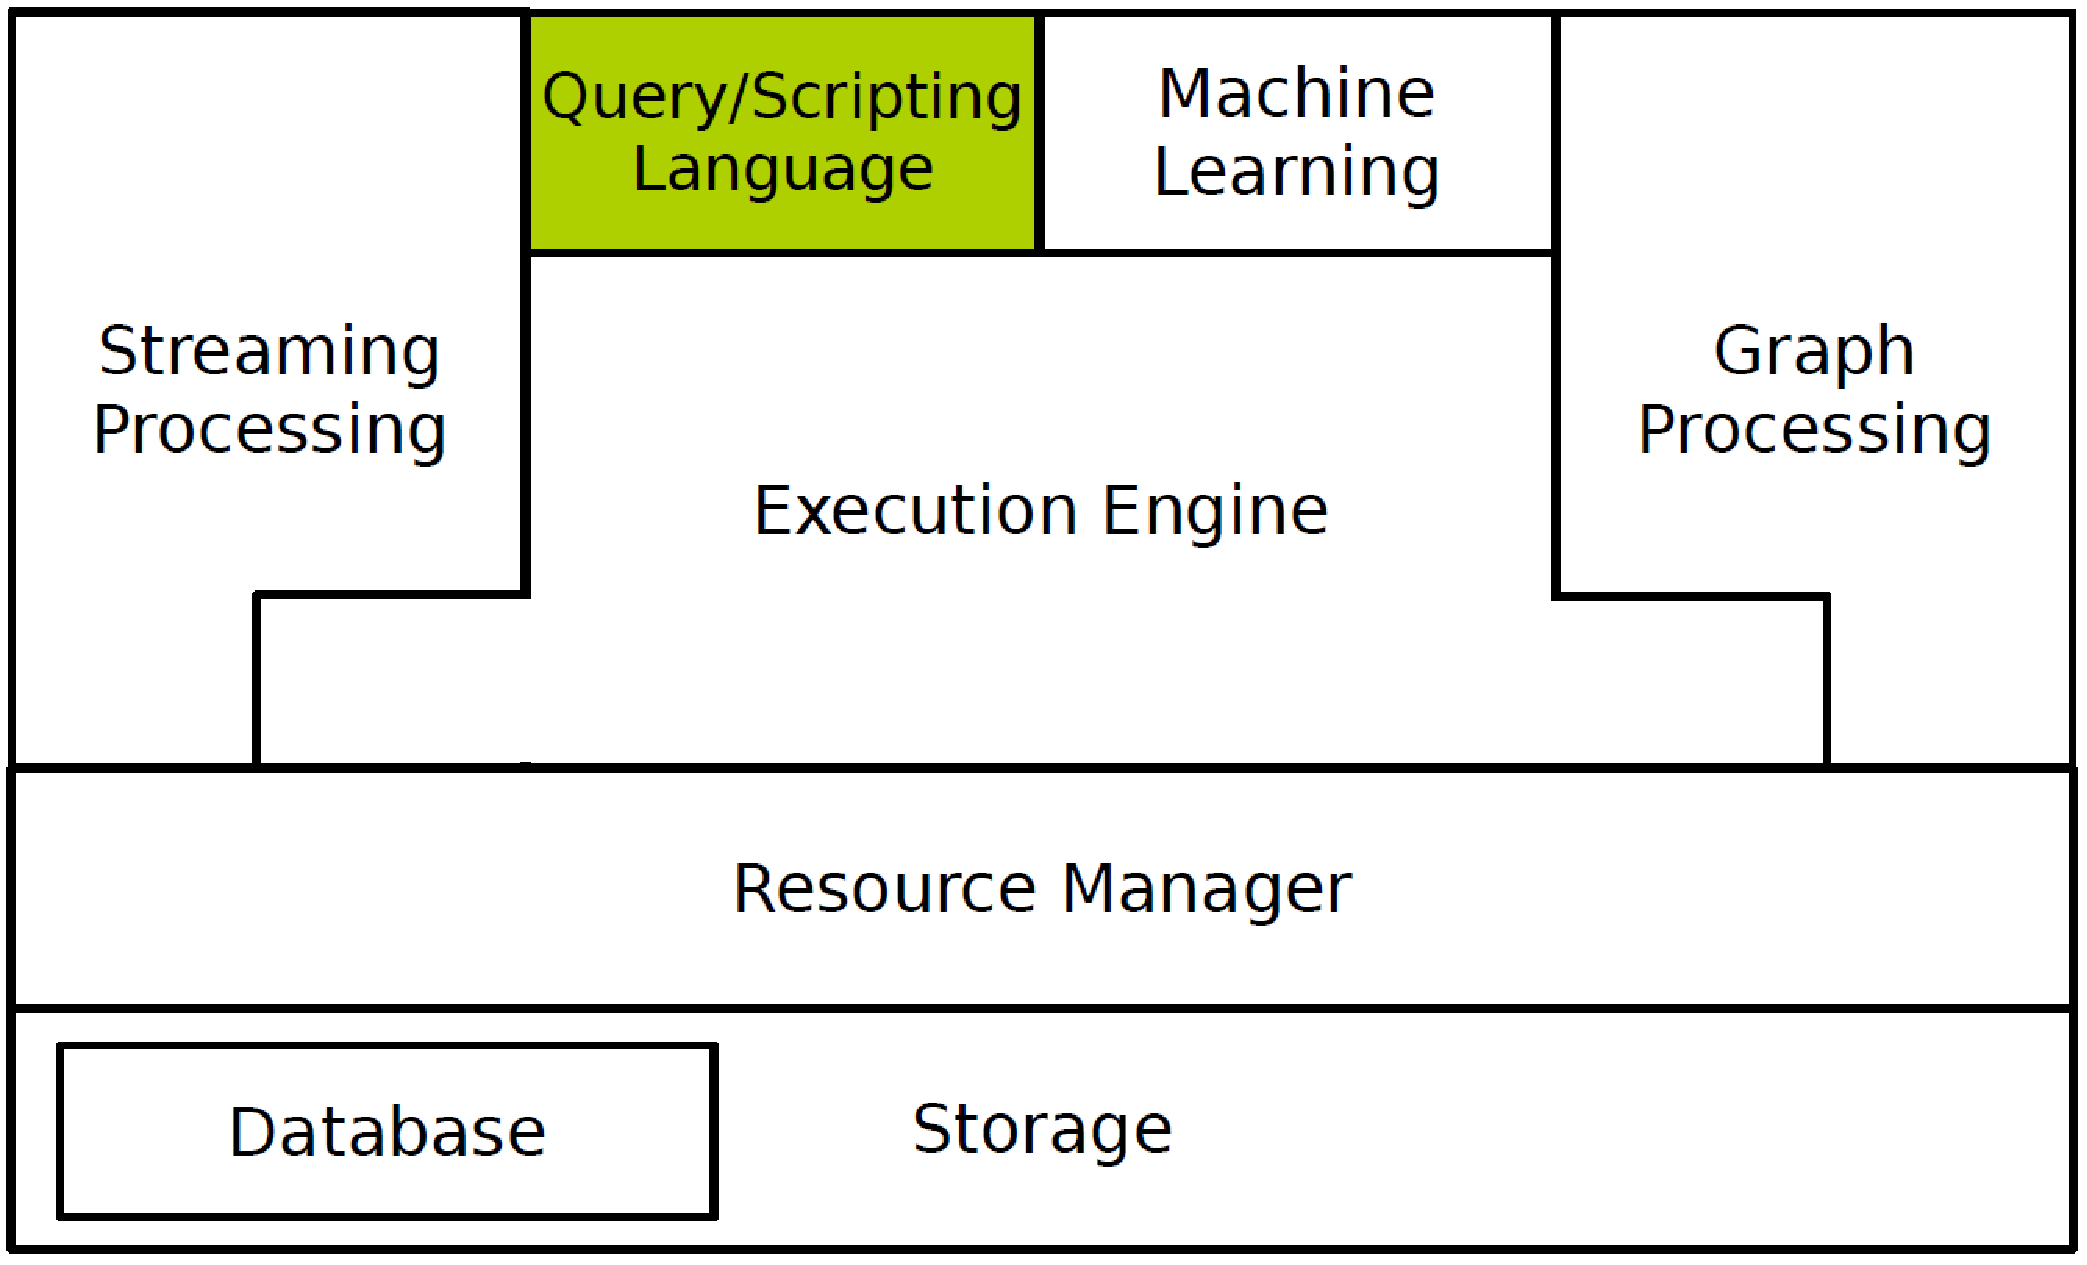
\includegraphics[width=2cm]{figs/stack_query.pdf}
\end{frame}

%------------------------------------------------
\begin{frame}
\frametitle{Big Data - Stream Processing}
\begin{columns}
\column{30em}
\begin{itemize}\itemsep1em
  \justifying
  \item Providing users with \textcolor{Ocean}{fresh} and \textcolor{Ocean}{low latency} results.
  \item Database Management Systems (\textcolor{TextGreen}{DBMS}) vs. Stream Processing Systems (\textcolor{TextGreen}{SPS})
  \vspace{0.3cm}
  \begin{columns}[c] 
  \column{.3\textwidth}
  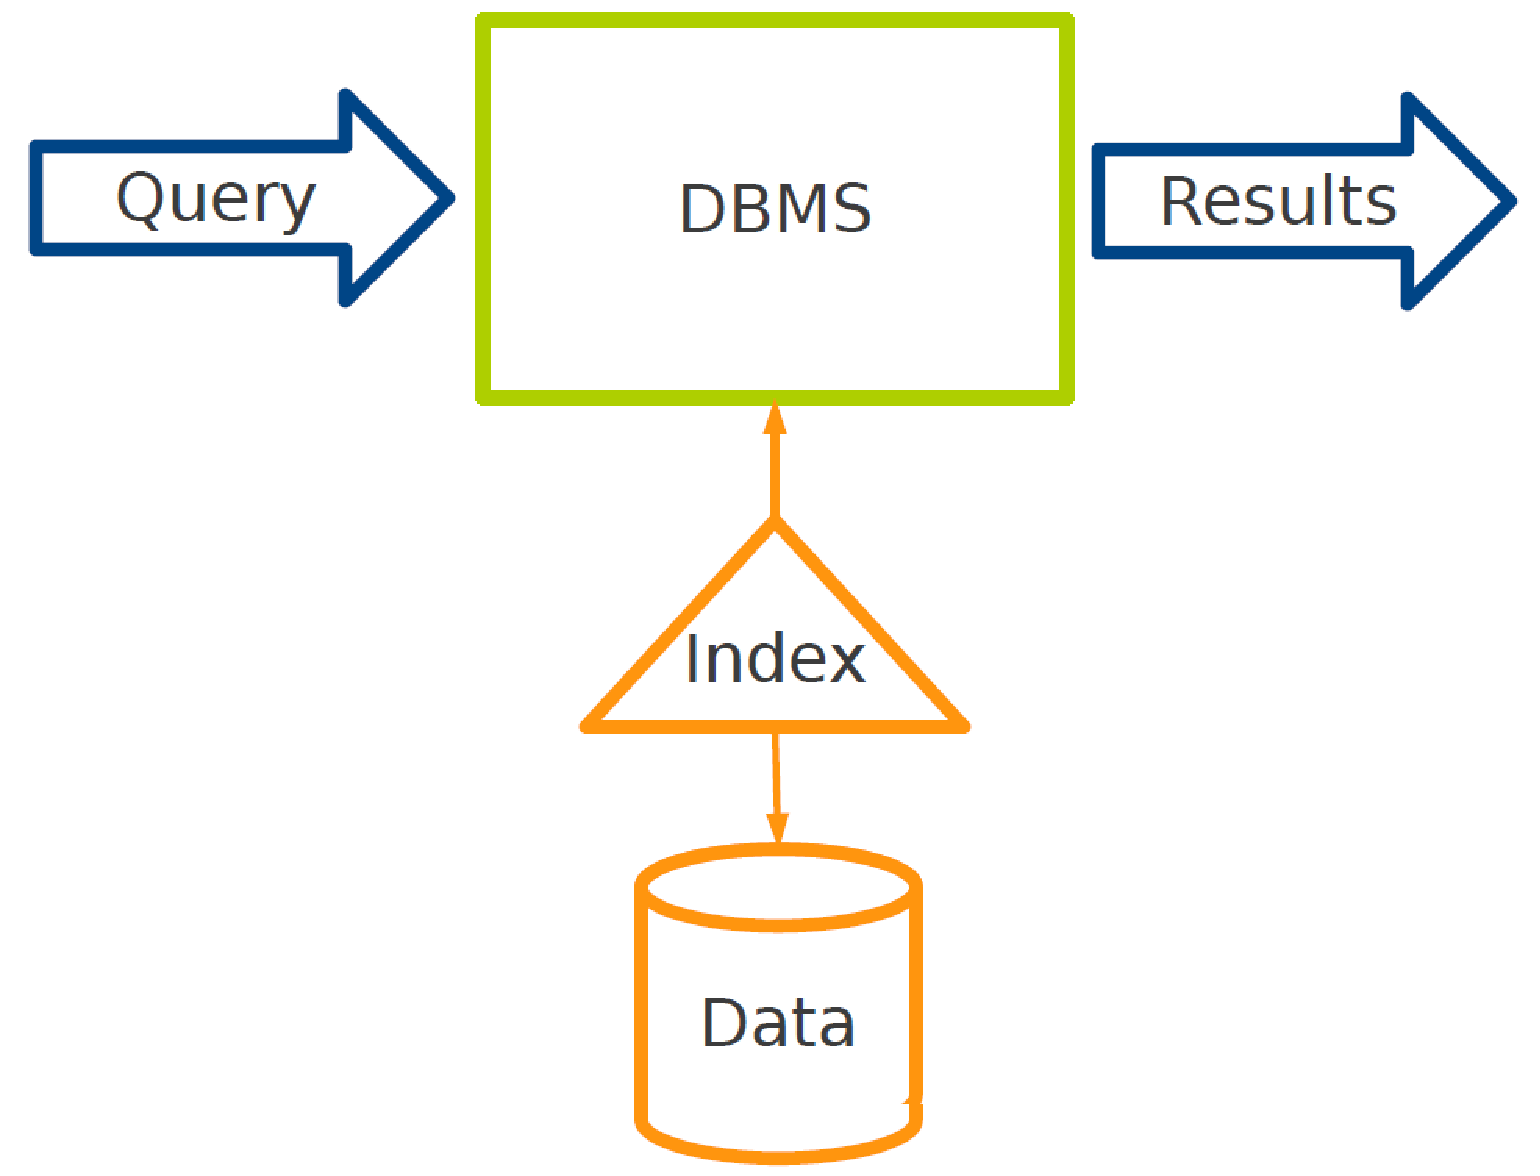
\includegraphics[width=3cm,valign=t]{figs/dbms.pdf}
  \column{.3\textwidth}
  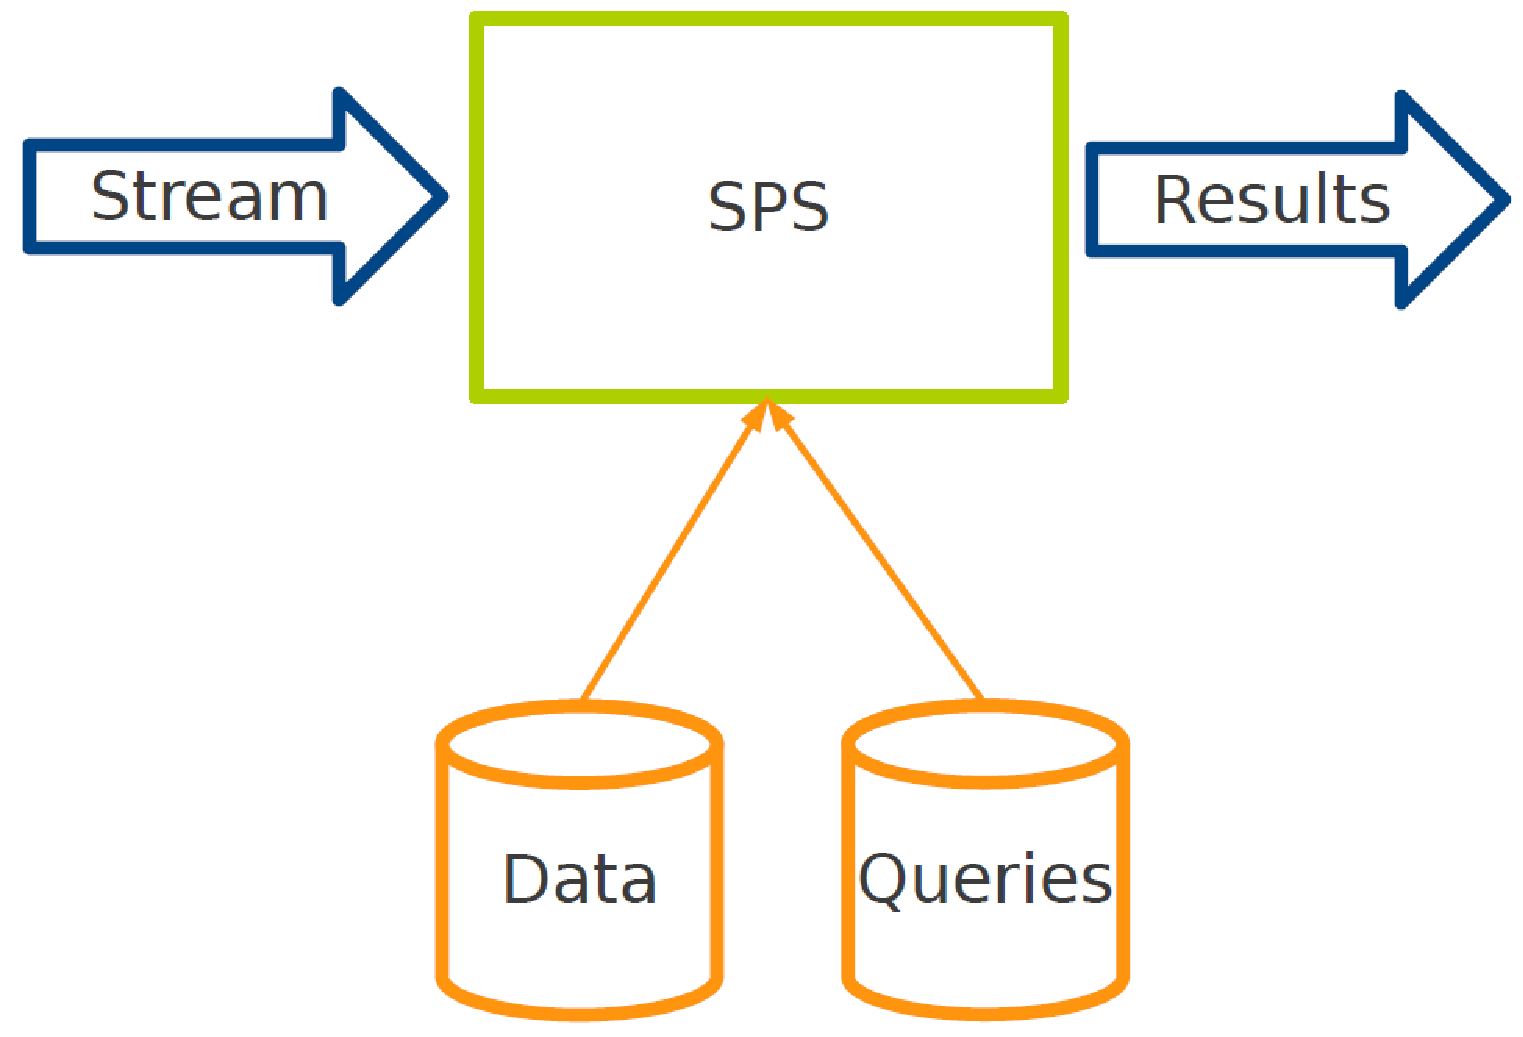
\includegraphics[width=3cm,valign=t]{figs/sps.pdf}
  \end{columns}
  \item Storm, S4, SEEP, D-Stream, Naiad, ...
\end{itemize}
\end{columns}
\vspace{0.62cm}
\hspace*{10cm}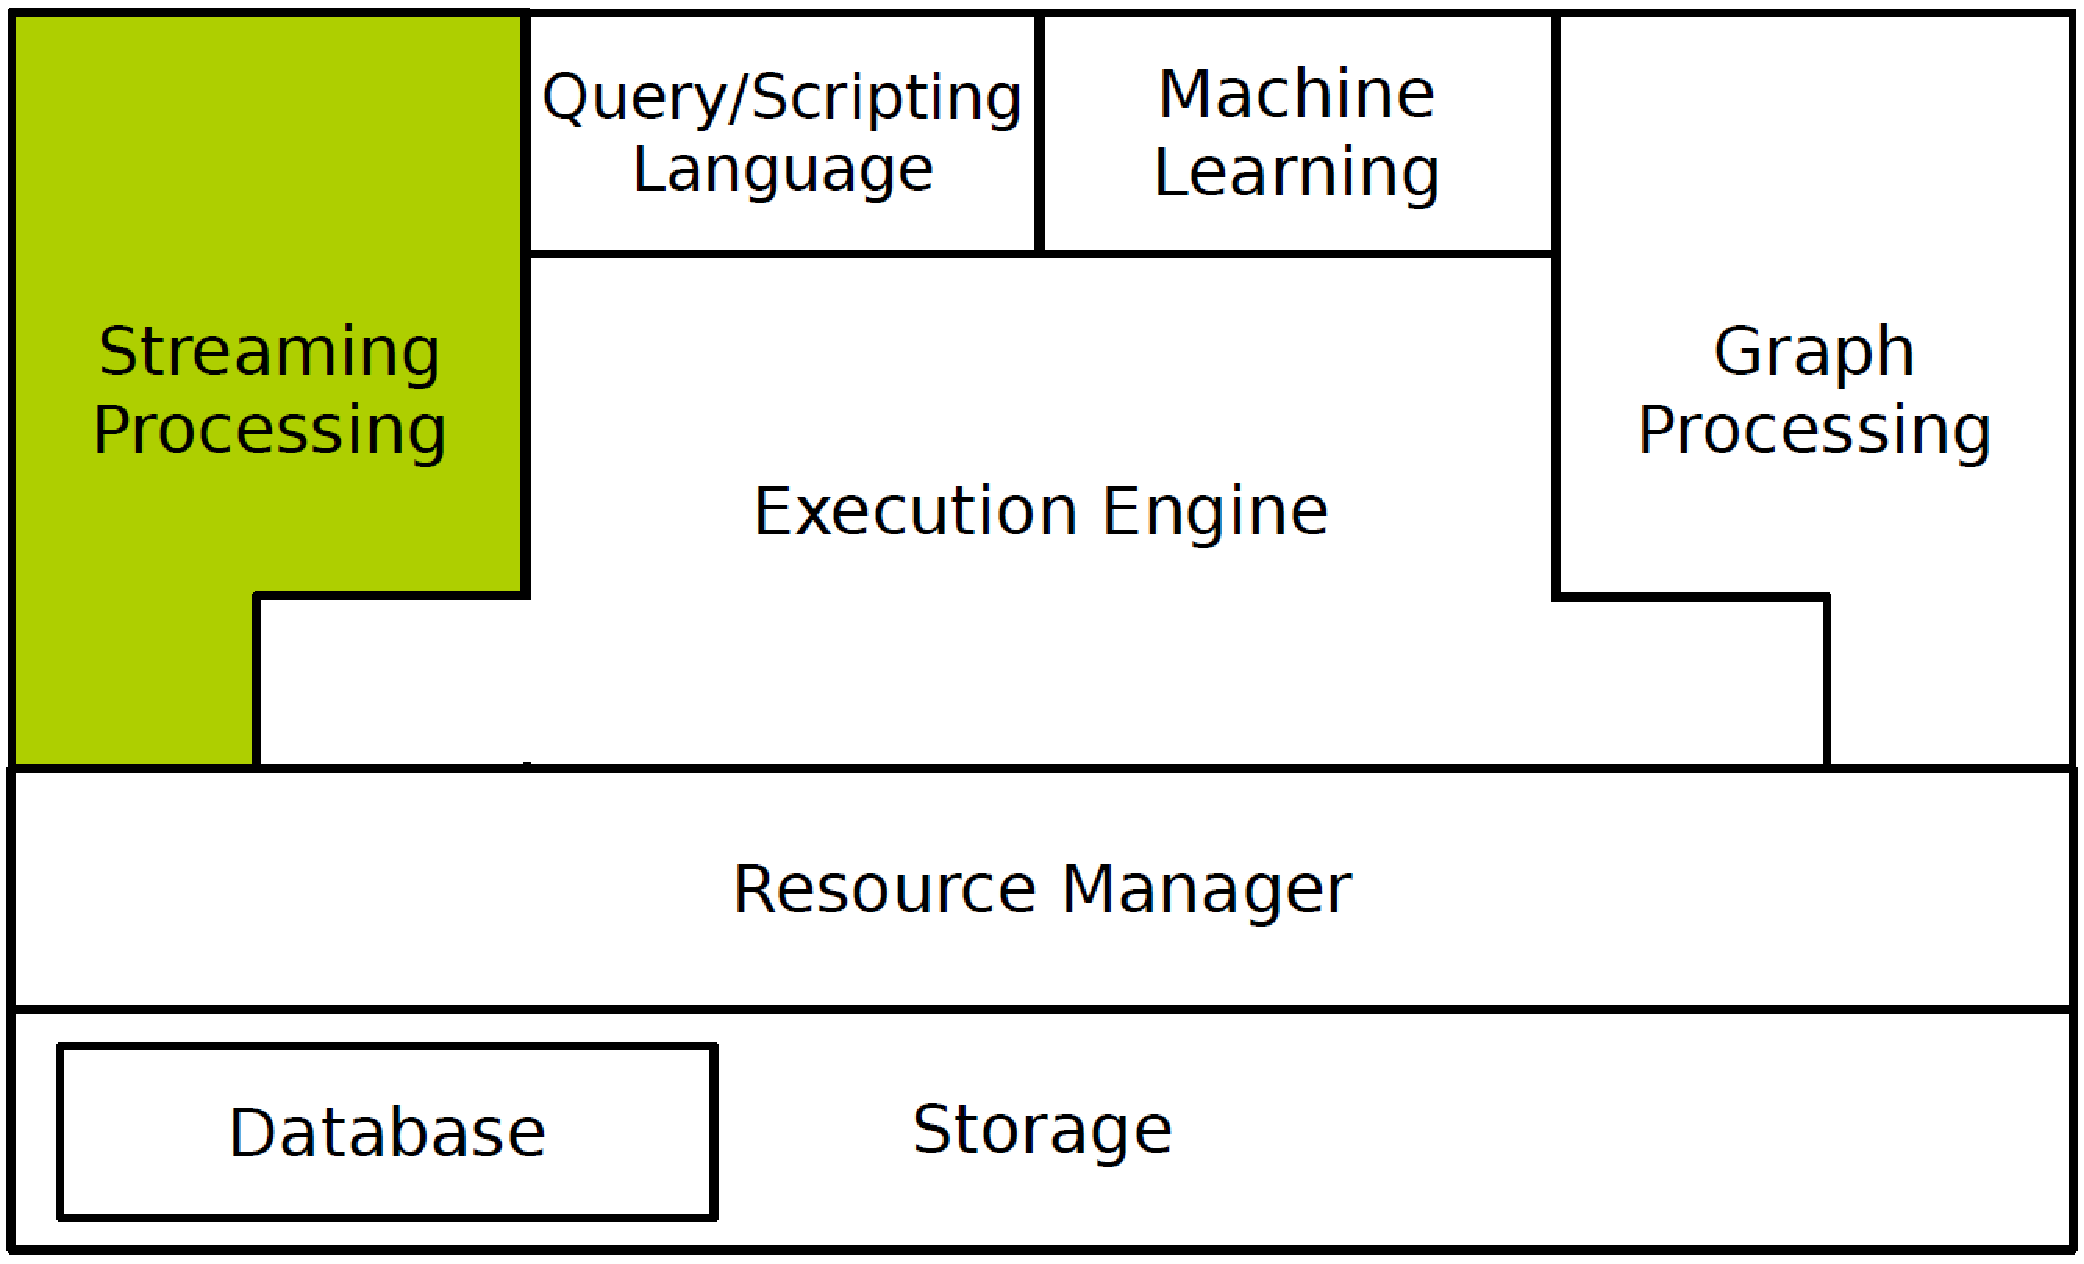
\includegraphics[width=2cm]{figs/stack_streaming.pdf}
\end{frame}

%------------------------------------------------
\begin{frame}
\frametitle{Big Data - Graph Processing}
\begin{columns}
\column{30em}
\begin{itemize}\itemsep1em
  \justifying
  \item Many problems are expressed using \textcolor{TextGreen}{graphs}: sparse \textcolor{Ocean}{computational dependencies}, and \textcolor{Ocean}{multiple iterations} to converge.
  \item Data-parallel frameworks, such as MapReduce, are not ideal for these problems: \textcolor{Ocean}{slow}
  \item Graph processing frameworks are \textcolor{Ocean}{optimized} for graph-based problems.
  \item Pregel, Giraph, GraphX, GraphLab, PowerGraph, GraphChi, ...
\end{itemize}
\end{columns}
\vspace{1.33cm}
\hspace*{10cm}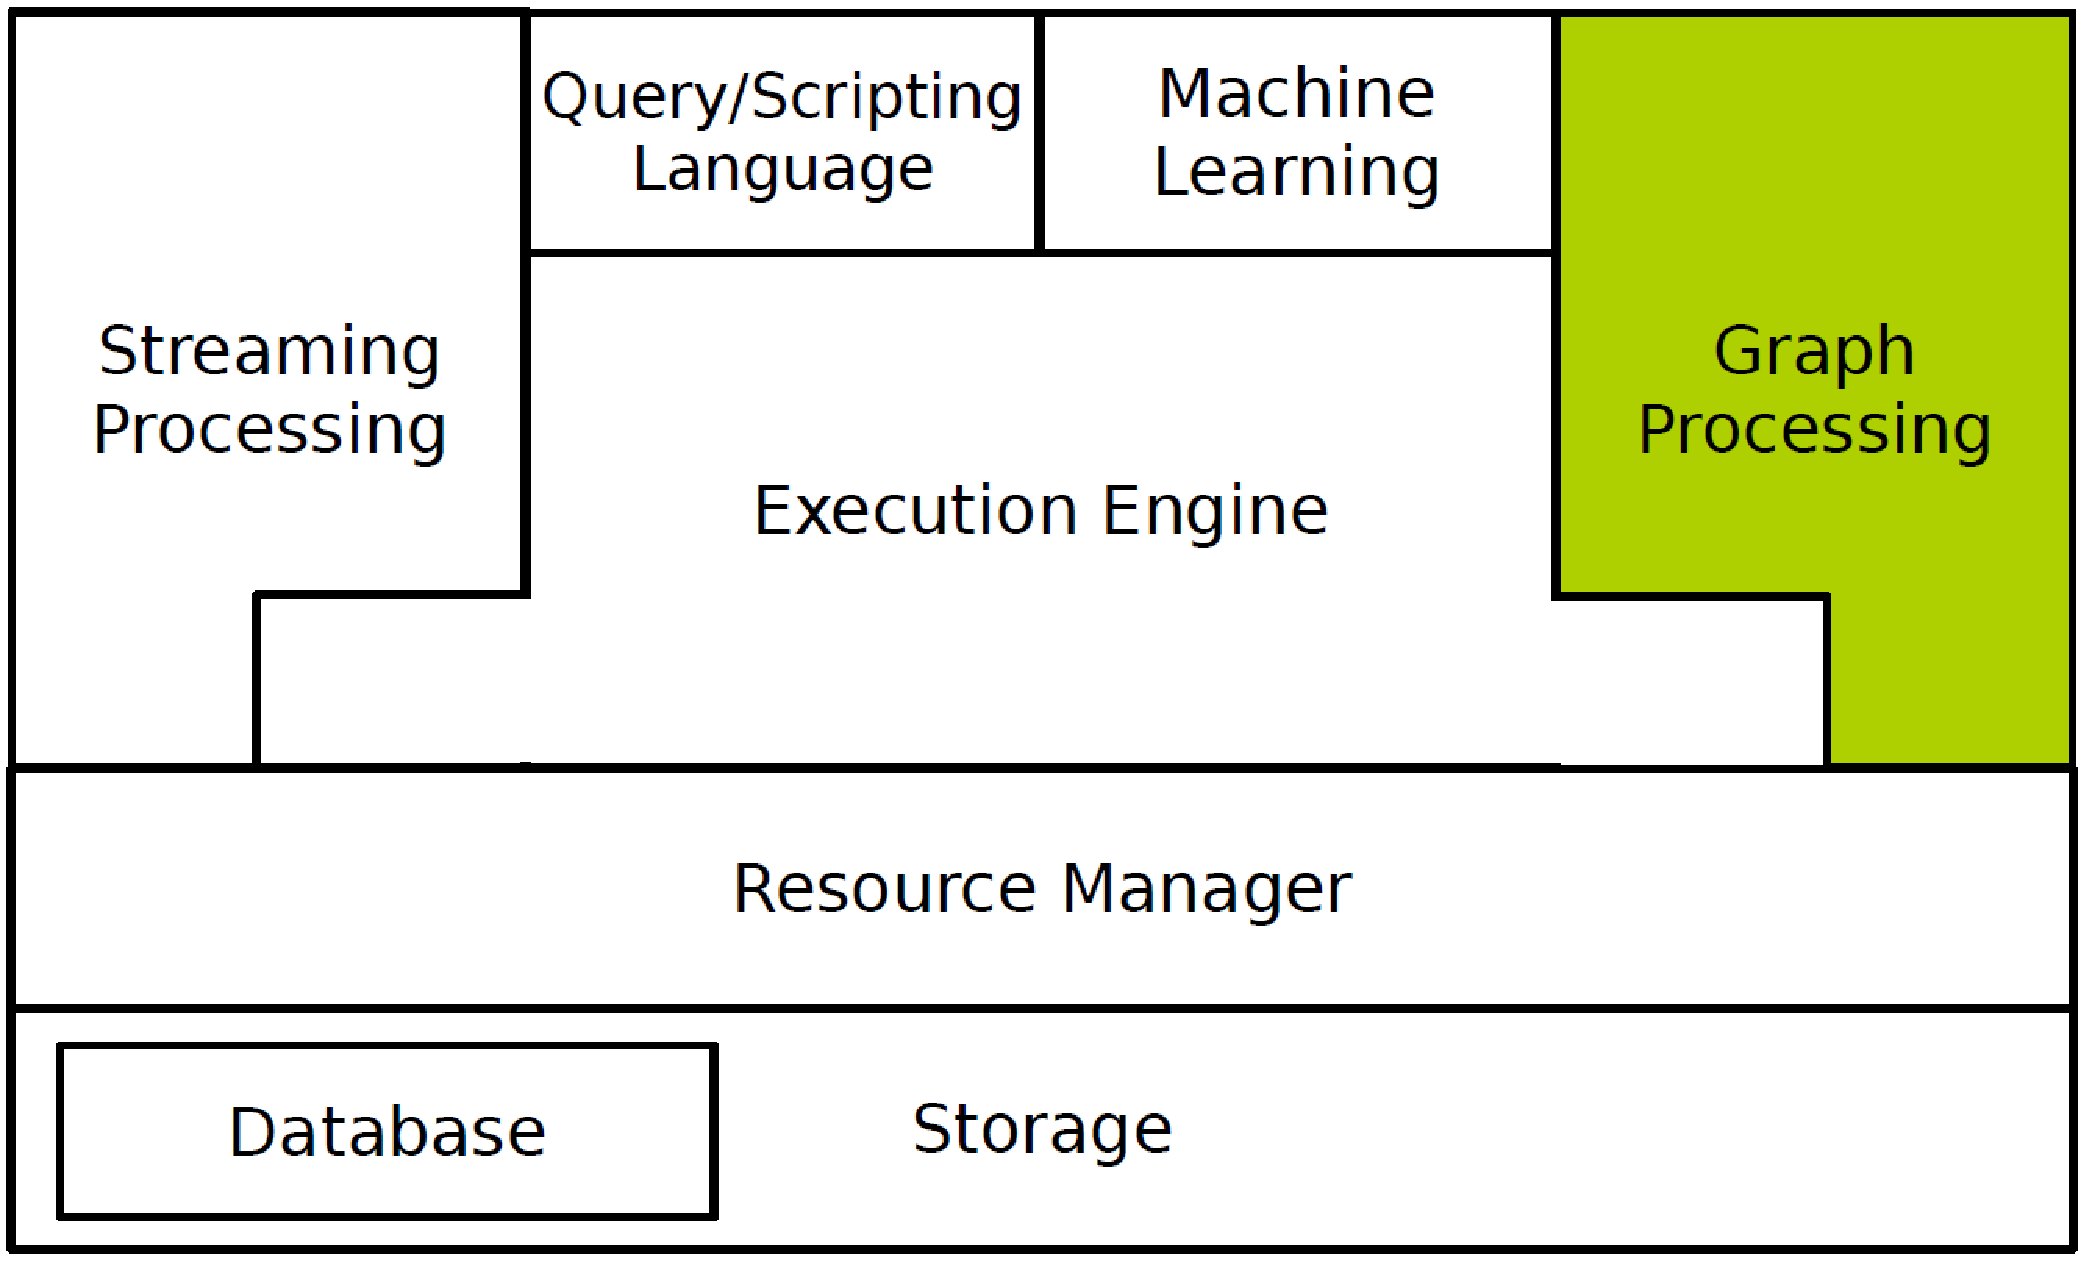
\includegraphics[width=2cm]{figs/stack_graph.pdf}
\end{frame}

%------------------------------------------------
\begin{frame}
\frametitle{Big Data - Machine Learning}
\begin{columns}
\column{30em}
\begin{itemize}\itemsep1em
  \justifying
  \item Implementing and consuming machine learning techniques at scale are \textcolor{Ocean}{difficult tasks} for developers and end users.
  \item There exist platforms that address it by providing scalable machine-learning and data mining libraries.
  \item Mahout, MLBase, SystemML, Ricardo, Presto, ...
\end{itemize}
\end{columns}
\vspace{2.67cm}
\hspace*{10cm}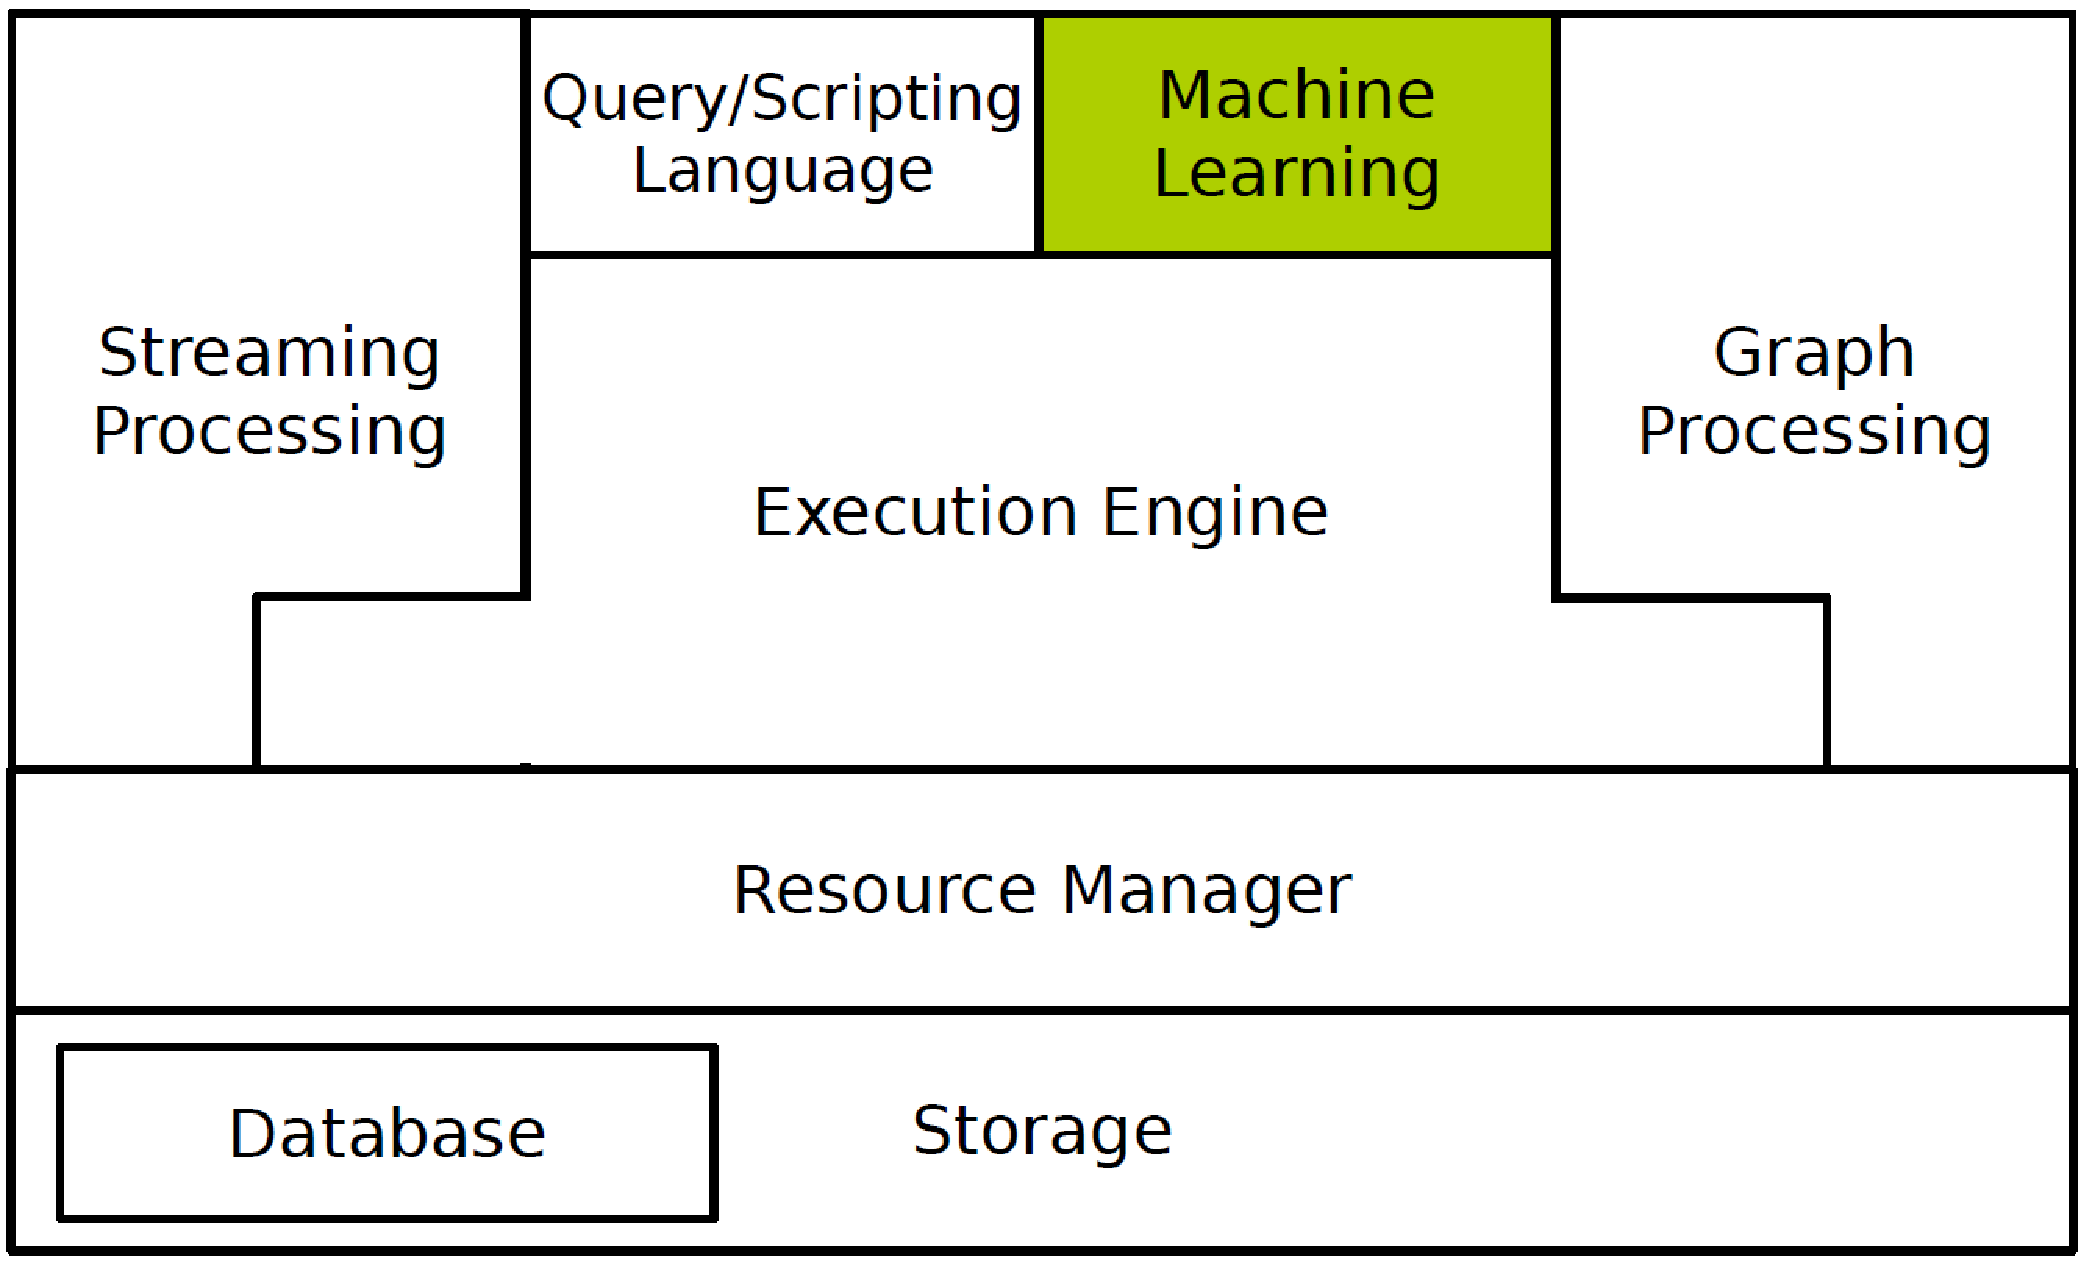
\includegraphics[width=2cm]{figs/stack_ml.pdf}
\end{frame}

%------------------------------------------------
\begin{frame}
\frametitle{Hadoop Big Data Analytics Stack}
\hspace*{4.7cm}
\includegraphics[width=2.5cm]{figs/hadoop.pdf}
\vspace{0.5cm}
\hspace*{3cm}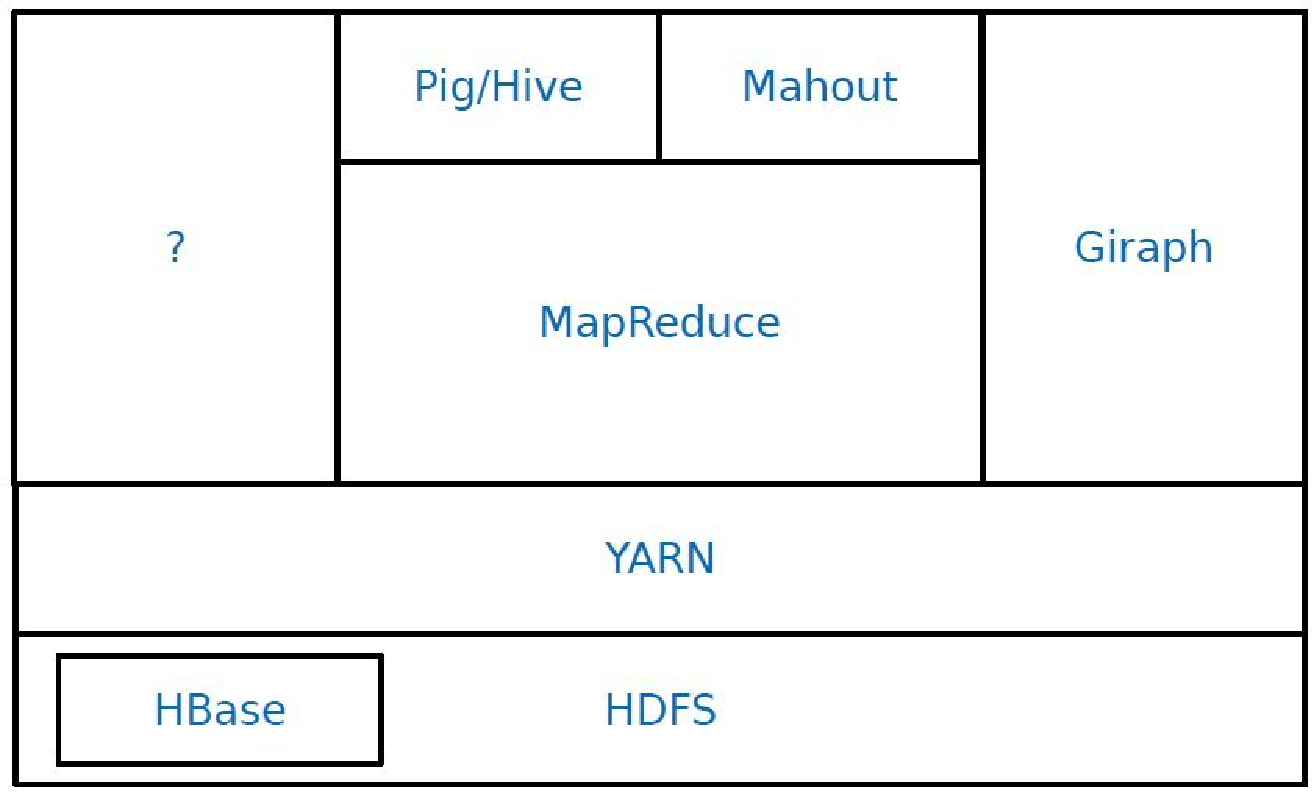
\includegraphics[width=6cm]{figs/stack_hadoop.pdf}
\end{frame}

%------------------------------------------------
\begin{frame}
\frametitle{Stratosphere Big Data Analytics Stack}
\hspace*{4.5cm}
\includegraphics[width=2.5cm]{figs/stratosphere.pdf}
\vspace{0.5cm}
\hspace*{3cm}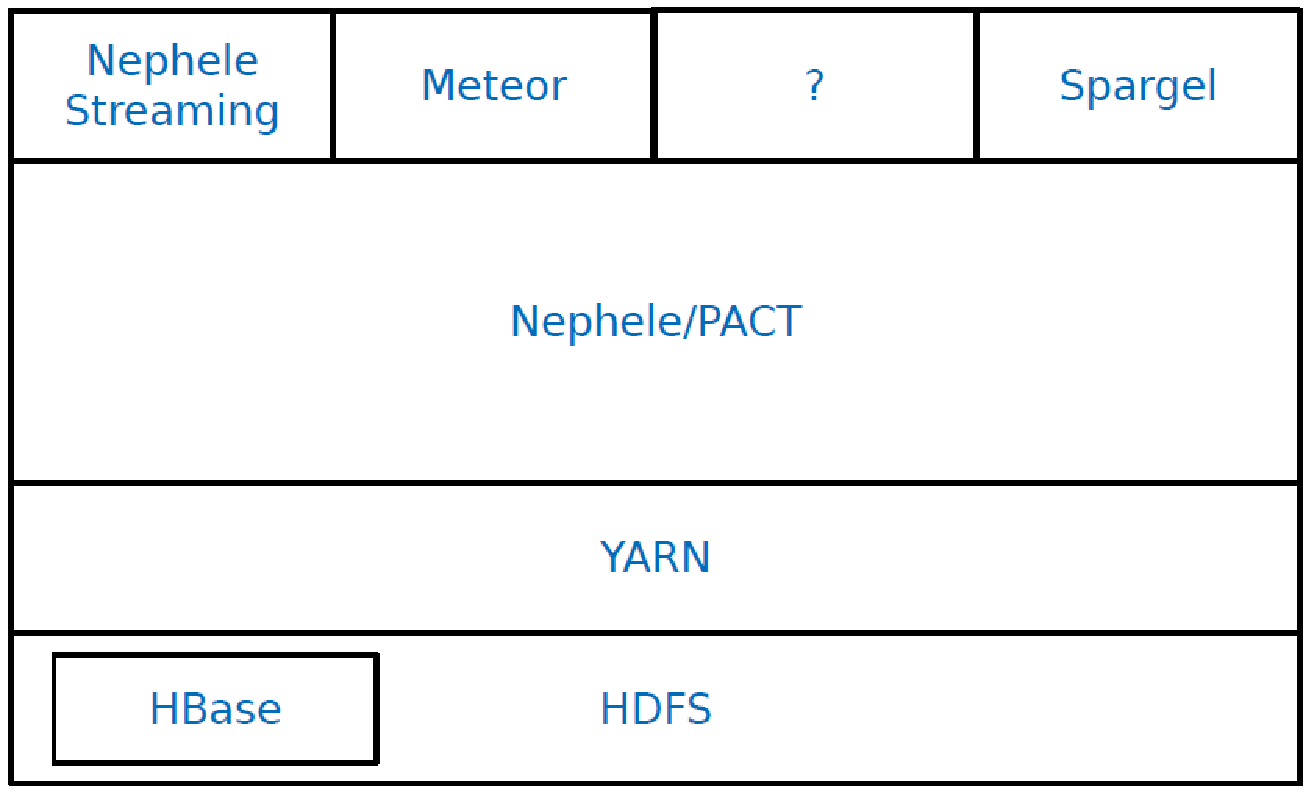
\includegraphics[width=6cm]{figs/stack_stratosphere.pdf}
\end{frame}

%------------------------------------------------
\begin{frame}
\frametitle{Spark Big Data Analytics Stack}
\hspace*{5cm}
\includegraphics[width=2cm]{figs/spark.pdf}
\vspace{0.5cm}
\hspace*{3cm}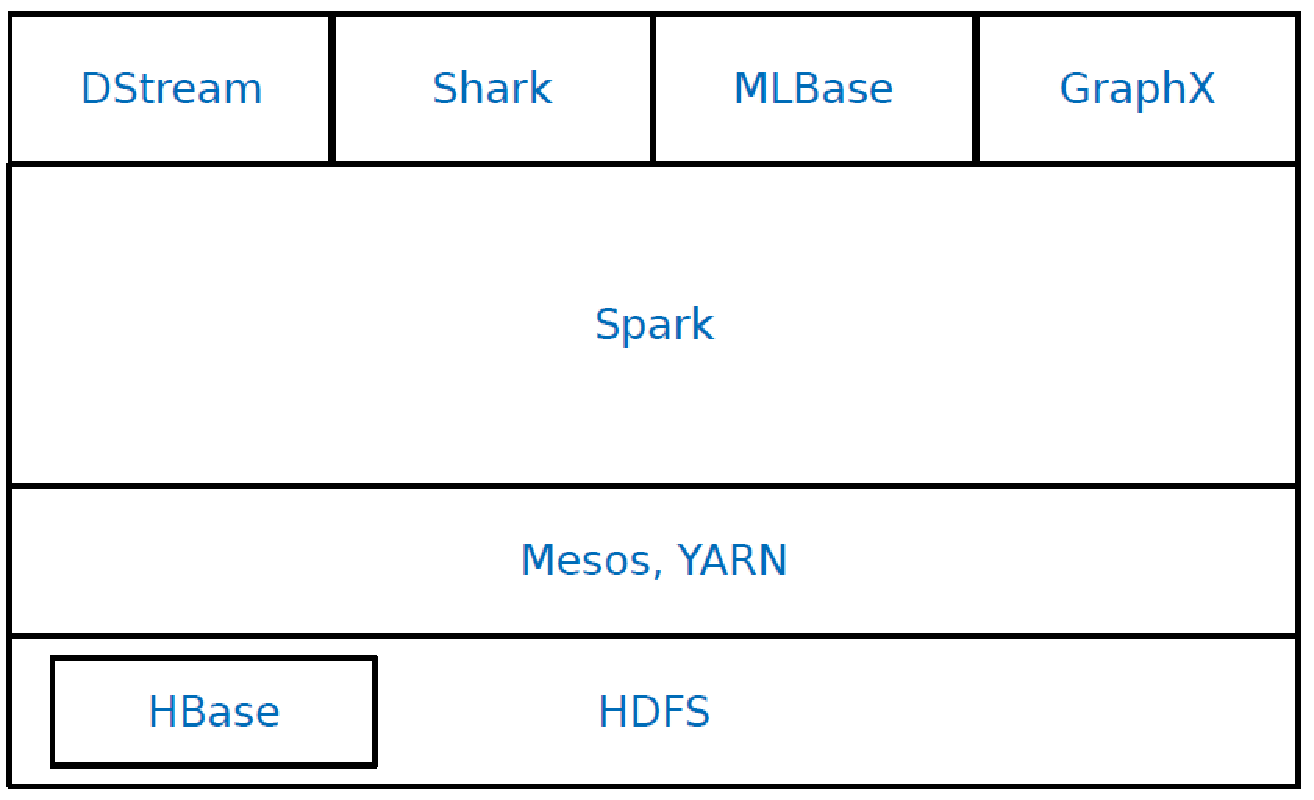
\includegraphics[width=6cm]{figs/stack_spark.pdf}
\end{frame}

%------------------------------------------------
\begin{frame}
\frametitle{Summary}
\hspace*{3cm}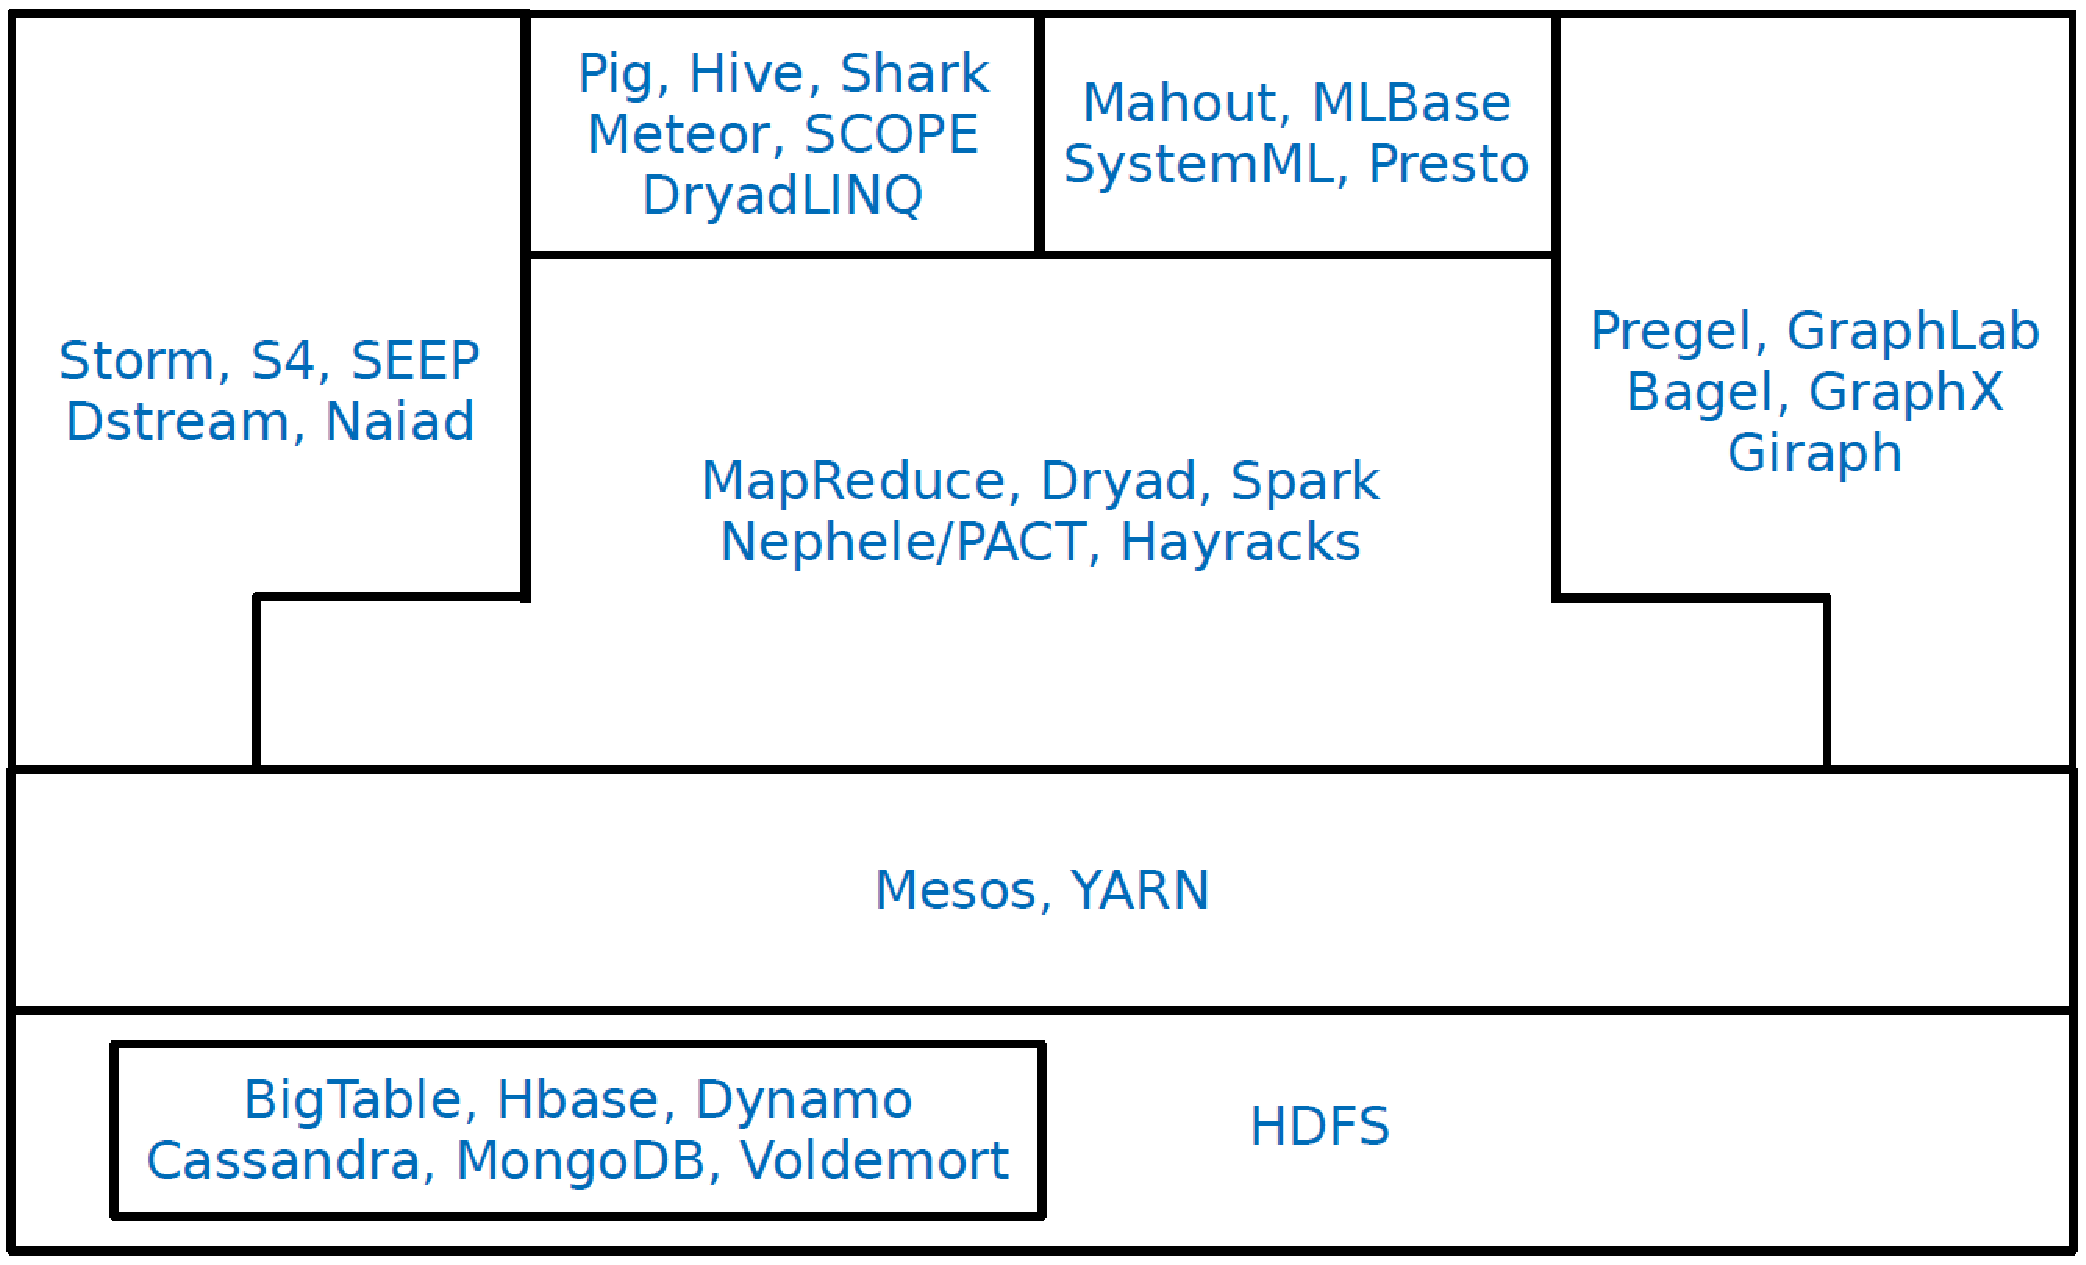
\includegraphics[width=6cm]{figs/summary.pdf}
\end{frame}

%------------------------------------------------
\begin{frame}
\vspace{1cm}
\Huge{\centerline{\usebeamercolor[fg]{title}Questions?}}
\end{frame}

\end{document} 